% Options for packages loaded elsewhere
\PassOptionsToPackage{unicode}{hyperref}
\PassOptionsToPackage{hyphens}{url}
\PassOptionsToPackage{dvipsnames,svgnames,x11names}{xcolor}
%
\documentclass[
]{article}

\usepackage{amsmath,amssymb}
\usepackage{iftex}
\ifPDFTeX
  \usepackage[T1]{fontenc}
  \usepackage[utf8]{inputenc}
  \usepackage{textcomp} % provide euro and other symbols
\else % if luatex or xetex
  \usepackage{unicode-math}
  \defaultfontfeatures{Scale=MatchLowercase}
  \defaultfontfeatures[\rmfamily]{Ligatures=TeX,Scale=1}
\fi
\usepackage{lmodern}
\ifPDFTeX\else  
    % xetex/luatex font selection
    \setmainfont[]{Latin Modern Roman}
  \setmathfont[]{Latin Modern Math}
\fi
% Use upquote if available, for straight quotes in verbatim environments
\IfFileExists{upquote.sty}{\usepackage{upquote}}{}
\IfFileExists{microtype.sty}{% use microtype if available
  \usepackage[]{microtype}
  \UseMicrotypeSet[protrusion]{basicmath} % disable protrusion for tt fonts
}{}
\makeatletter
\@ifundefined{KOMAClassName}{% if non-KOMA class
  \IfFileExists{parskip.sty}{%
    \usepackage{parskip}
  }{% else
    \setlength{\parindent}{0pt}
    \setlength{\parskip}{6pt plus 2pt minus 1pt}}
}{% if KOMA class
  \KOMAoptions{parskip=half}}
\makeatother
\usepackage{xcolor}
\setlength{\emergencystretch}{3em} % prevent overfull lines
\setcounter{secnumdepth}{5}
% Make \paragraph and \subparagraph free-standing
\makeatletter
\ifx\paragraph\undefined\else
  \let\oldparagraph\paragraph
  \renewcommand{\paragraph}{
    \@ifstar
      \xxxParagraphStar
      \xxxParagraphNoStar
  }
  \newcommand{\xxxParagraphStar}[1]{\oldparagraph*{#1}\mbox{}}
  \newcommand{\xxxParagraphNoStar}[1]{\oldparagraph{#1}\mbox{}}
\fi
\ifx\subparagraph\undefined\else
  \let\oldsubparagraph\subparagraph
  \renewcommand{\subparagraph}{
    \@ifstar
      \xxxSubParagraphStar
      \xxxSubParagraphNoStar
  }
  \newcommand{\xxxSubParagraphStar}[1]{\oldsubparagraph*{#1}\mbox{}}
  \newcommand{\xxxSubParagraphNoStar}[1]{\oldsubparagraph{#1}\mbox{}}
\fi
\makeatother


\providecommand{\tightlist}{%
  \setlength{\itemsep}{0pt}\setlength{\parskip}{0pt}}\usepackage{longtable,booktabs,array}
\usepackage{calc} % for calculating minipage widths
% Correct order of tables after \paragraph or \subparagraph
\usepackage{etoolbox}
\makeatletter
\patchcmd\longtable{\par}{\if@noskipsec\mbox{}\fi\par}{}{}
\makeatother
% Allow footnotes in longtable head/foot
\IfFileExists{footnotehyper.sty}{\usepackage{footnotehyper}}{\usepackage{footnote}}
\makesavenoteenv{longtable}
\usepackage{graphicx}
\makeatletter
\newsavebox\pandoc@box
\newcommand*\pandocbounded[1]{% scales image to fit in text height/width
  \sbox\pandoc@box{#1}%
  \Gscale@div\@tempa{\textheight}{\dimexpr\ht\pandoc@box+\dp\pandoc@box\relax}%
  \Gscale@div\@tempb{\linewidth}{\wd\pandoc@box}%
  \ifdim\@tempb\p@<\@tempa\p@\let\@tempa\@tempb\fi% select the smaller of both
  \ifdim\@tempa\p@<\p@\scalebox{\@tempa}{\usebox\pandoc@box}%
  \else\usebox{\pandoc@box}%
  \fi%
}
% Set default figure placement to htbp
\def\fps@figure{htbp}
\makeatother
% definitions for citeproc citations
\NewDocumentCommand\citeproctext{}{}
\NewDocumentCommand\citeproc{mm}{%
  \begingroup\def\citeproctext{#2}\cite{#1}\endgroup}
\makeatletter
 % allow citations to break across lines
 \let\@cite@ofmt\@firstofone
 % avoid brackets around text for \cite:
 \def\@biblabel#1{}
 \def\@cite#1#2{{#1\if@tempswa , #2\fi}}
\makeatother
\newlength{\cslhangindent}
\setlength{\cslhangindent}{1.5em}
\newlength{\csllabelwidth}
\setlength{\csllabelwidth}{3em}
\newenvironment{CSLReferences}[2] % #1 hanging-indent, #2 entry-spacing
 {\begin{list}{}{%
  \setlength{\itemindent}{0pt}
  \setlength{\leftmargin}{0pt}
  \setlength{\parsep}{0pt}
  % turn on hanging indent if param 1 is 1
  \ifodd #1
   \setlength{\leftmargin}{\cslhangindent}
   \setlength{\itemindent}{-1\cslhangindent}
  \fi
  % set entry spacing
  \setlength{\itemsep}{#2\baselineskip}}}
 {\end{list}}
\usepackage{calc}
\newcommand{\CSLBlock}[1]{\hfill\break\parbox[t]{\linewidth}{\strut\ignorespaces#1\strut}}
\newcommand{\CSLLeftMargin}[1]{\parbox[t]{\csllabelwidth}{\strut#1\strut}}
\newcommand{\CSLRightInline}[1]{\parbox[t]{\linewidth - \csllabelwidth}{\strut#1\strut}}
\newcommand{\CSLIndent}[1]{\hspace{\cslhangindent}#1}

\usepackage{arxiv}
\usepackage{orcidlink}
\usepackage{amsmath}
\usepackage[T1]{fontenc}
\makeatletter
\@ifpackageloaded{caption}{}{\usepackage{caption}}
\AtBeginDocument{%
\ifdefined\contentsname
  \renewcommand*\contentsname{Table of contents}
\else
  \newcommand\contentsname{Table of contents}
\fi
\ifdefined\listfigurename
  \renewcommand*\listfigurename{List of Figures}
\else
  \newcommand\listfigurename{List of Figures}
\fi
\ifdefined\listtablename
  \renewcommand*\listtablename{List of Tables}
\else
  \newcommand\listtablename{List of Tables}
\fi
\ifdefined\figurename
  \renewcommand*\figurename{Figure}
\else
  \newcommand\figurename{Figure}
\fi
\ifdefined\tablename
  \renewcommand*\tablename{Table}
\else
  \newcommand\tablename{Table}
\fi
}
\@ifpackageloaded{float}{}{\usepackage{float}}
\floatstyle{ruled}
\@ifundefined{c@chapter}{\newfloat{codelisting}{h}{lop}}{\newfloat{codelisting}{h}{lop}[chapter]}
\floatname{codelisting}{Listing}
\newcommand*\listoflistings{\listof{codelisting}{List of Listings}}
\makeatother
\makeatletter
\makeatother
\makeatletter
\@ifpackageloaded{caption}{}{\usepackage{caption}}
\@ifpackageloaded{subcaption}{}{\usepackage{subcaption}}
\makeatother

\usepackage{bookmark}

\IfFileExists{xurl.sty}{\usepackage{xurl}}{} % add URL line breaks if available
\urlstyle{same} % disable monospaced font for URLs
\hypersetup{
  pdftitle={Clinical Language Encoding with ModernBERT},
  pdfauthor={Tyler M Cross},
  pdfkeywords={clinical natural language
processing, ModernBERT, MIMIC-IV, MIMIC-III, MDACE, multi-label
classification},
  colorlinks=true,
  linkcolor={blue},
  filecolor={Maroon},
  citecolor={Blue},
  urlcolor={Blue},
  pdfcreator={LaTeX via pandoc}}


\newcommand{\runninghead}{A Preprint }
\renewcommand{\runninghead}{A Preprint }
\title{Clinical Language Encoding with ModernBERT}
\def\asep{\\\\\\ } % default: all authors on same column
\author{\textbf{Tyler M Cross}~\orcidlink{0009-0003-3529-8222}\\Master's
in Data Science\\University of California, Berkeley School of
Information\\Berkeley,
CA,\ 94720\\\href{mailto:tyler.cross@berkeley.edu}{tyler.cross@berkeley.edu}}
\date{}
\begin{document}
\maketitle
\begin{abstract}
Medical coding---assigning standardized codes to clinical
documentation---is a costly, labor-intensive process. Automating this
task via multi-label classification faces challenges like long documents
and extreme class imbalance. We present CLEM-ICD, replacing the
RoBERTa/BERT base models common in prior frameworks with ModernBERT,
leveraging its 8192-token context window to better process lengthy
clinical notes. ModernBERT's optimized architecture (\textasciitilde138M
parameters) enhances computational efficiency and simplifies
implementation compared to prior approaches requiring complex
modifications for shorter-context models. Evaluating on the MDACE
dataset, CLEM-ICD achieves a Micro-F1 score of 47.6\%, outperforming
recent results by Edin et al. (2024) (41.9\% Micro-F1). On the standard
MIMIC-III benchmark, CLEM-ICD achieves a notably high Macro-F1 of
16.5\%, significantly outperforming the current state-of-the-art on
uncommon classes. CLEM-ICD demonstrates how modern architectural
advancements, particularly large context windows applied to encoder-only
models, can yield strong performance on complex tasks like automated
medical coding. We release our code and models to foster further
research.
\end{abstract}
{\bfseries \emph Keywords}
\def\sep{\textbullet\ }
clinical natural language
processing \sep ModernBERT \sep MIMIC-IV \sep MIMIC-III \sep MDACE \sep 
multi-label classification



\section{Introduction}\label{sec-intro}

Medical coding, the assignment of standardized codes to clinical
documentation, is an essential step for medical billing and
reimbursement. The administrative processes surrounding billing and
insurance-related activities, which heavily rely on accurate coding,
represent a significant burden, consuming up to 25\% of healthcare
expenditures in the United States (Kocher and Sahni 2011; Tseng et al.
2018). Research has focused on attempts to automate coding by training
multi-label classification models, with transformer-based architectures
emerging as particularly effective (Huang, Tsai, and Chen 2022; Liu et
al. 2024). The PLM-ICD framework (Huang, Tsai, and Chen 2022), utilizing
BERT-based language models to encode clinical documents, established a
strong benchmark for automated ICD coding by effectively balancing model
complexity and predictive accuracy on the MIMIC-III dataset (A. E.
Johnson et al. 2016).

Despite advances, significant challenges persist in automated medical
coding systems. Clinical documents often exceed the standard context
windows (e.g., 512 tokens) of many transformer models, causing potential
information loss during truncation or requiring complex workarounds like
the segment pooling employed by PLM-ICD (Huang, Tsai, and Chen 2022).
Furthermore, the extreme class imbalance inherent in ICD coding hinders
performance on rare but clinically significant codes. Although
transformer-based approaches generally outperform older convolutional
and recurrent architectures, these limitations highlight the need for
architectures with natively expanded context windows, a capability
offered by modern transformer variants like ModernBERT (Warner et al.
2024), which can process lengthy clinical documents more holistically.

\section{Methods}\label{sec-methods}

We followed the established data preparation pipeline developed by Cheng
et al. (2023) for processing the MIMIC-III and MIMIC-IV datasets (A. E.
W. Johnson et al. 2023), heavily relying on the open-source code
provided by Edin et al. (2024) to match clinical visit notes with their
associated diagnostic and procedure codes. Specifically, for the results
compared against Edin et al. (2024) in Table~\ref{tbl-results}, we
utilized the MIMIC-III dataset (A. E. Johnson et al. 2016), focusing on
inpatient discharge summaries and their associated ICD-9 codes,
processed according to the splits defined by Cheng et al. (2023). These
notes originate from various clinicians across intensive care units at
the Beth Israel Deaconess Medical Center. While previous approaches like
PLM-ICD (Huang, Tsai, and Chen 2022) and its iterations employed
specialized architectures for clinical text encoding, we diverged from
this approach by adopting the more generic multi-label classification
architecture recommended by ModernBERT (Warner et al. 2024). This
decision simplified the architecture, facilitating experimentation and
fully leveraging ModernBERT's 8192-token context window.

Training transformer models with such extended context windows presented
significant computational challenges, particularly on consumer-grade
hardware. To address memory constraints, we implemented a combination of
gradient checkpointing during backpropagation and Flash Attention 2.0
(Dao et al. 2022). These optimizations enabled us to train our models on
a standard consumer GPU without degrading performance. To facilitate
direct comparison with existing approaches, we attempted to maintain the
same evaluation metrics employed by PLM-ICD and subsequent works (Huang,
Tsai, and Chen 2022; Edin et al. 2024; Liu et al. 2024), including micro
and macro-averaged F1 scores, precision, and recall metrics, which
represent the standard evaluation framework in this field.

\section{Results}\label{sec-results}

Our proposed CLEM-ICD model, leveraging the ModernBERT architecture with
an 8192-token context window, was evaluated on the MDACE dataset using
the standard multi-label classification metrics. The best performing
model achieved a Micro-averaged F1 score (Micro-F1) of 0.476,
Micro-Precision of 0.680, and Micro-Recall of 0.366 on the test set. The
Macro-averaged F1 score (Macro-F1) reached 0.038.

\begin{longtable}[]{@{}
  >{\raggedright\arraybackslash}p{(\linewidth - 6\tabcolsep) * \real{0.4875}}
  >{\raggedright\arraybackslash}p{(\linewidth - 6\tabcolsep) * \real{0.1875}}
  >{\raggedright\arraybackslash}p{(\linewidth - 6\tabcolsep) * \real{0.1500}}
  >{\raggedright\arraybackslash}p{(\linewidth - 6\tabcolsep) * \real{0.1750}}@{}}
\caption{Comparison of multi-label classification performance metrics
between our CLEM-ICD model and the AttInGrad (TM) baseline from Edin et
al. (2024).}\label{tbl-results}\tabularnewline
\toprule\noalign{}
\begin{minipage}[b]{\linewidth}\raggedright
Model
\end{minipage} & \begin{minipage}[b]{\linewidth}\raggedright
Precision (\%)
\end{minipage} & \begin{minipage}[b]{\linewidth}\raggedright
Recall (\%)
\end{minipage} & \begin{minipage}[b]{\linewidth}\raggedright
Micro-F1 (\%)
\end{minipage} \\
\midrule\noalign{}
\endfirsthead
\toprule\noalign{}
\begin{minipage}[b]{\linewidth}\raggedright
Model
\end{minipage} & \begin{minipage}[b]{\linewidth}\raggedright
Precision (\%)
\end{minipage} & \begin{minipage}[b]{\linewidth}\raggedright
Recall (\%)
\end{minipage} & \begin{minipage}[b]{\linewidth}\raggedright
Micro-F1 (\%)
\end{minipage} \\
\midrule\noalign{}
\endhead
\bottomrule\noalign{}
\endlastfoot
AttInGrad (TM) (Edin et al. 2024) & 40.2 \(\pm\) 3.0 & 43.9 \(\pm\) 4.8
& 41.9 \(\pm\) 3.4 \\
CLEM-ICD (Ours) & 68.0 & 36.6 & 47.6 \\
\end{longtable}

These results demonstrate a notable improvement over recent benchmarks.
For instance, comparing our Micro-F1 score of 47.6\% to the 41.9\%
reported by Edin et al. (2024) for their AttInGrad model on the same
MIMIC-III/MDACE benchmark dataset, our approach shows enhanced
performance. A key difference is that the Edin et al. (2024) results are
averaged over 10 runs, providing confidence intervals, whereas our
CLEM-ICD results are based on a single training run due to computational
constraints. Nevertheless, the CLEM-ICD model appears competitive with,
and potentially surpasses, state-of-the-art methods like PLM-ICD (Huang,
Tsai, and Chen 2022) under similar evaluation conditions, particularly
benefiting from the extended context capacity. The low Macro-F1 score
(3.8\% on this dataset), however, aligns with observations in prior
work, indicating persistent challenges in accurately classifying less
frequent codes within the highly imbalanced ICD code distribution.

To provide a direct comparison on the widely used MIMIC-III benchmark
dataset (A. E. Johnson et al. 2016), we evaluate CLEM-ICD against the
original PLM-ICD (Huang, Tsai, and Chen 2022) and subsequent
improvements reported by Liu et al. (2024). The results are summarized
in Table~\ref{tbl-mimic3-comparison}. Our CLEM-ICD model demonstrates a
strong Macro-F1 score, suggesting better performance on less frequent
codes compared to prior work, although the Micro-F1 score is lower in
this specific run.

\begin{longtable}[]{@{}
  >{\raggedright\arraybackslash}p{(\linewidth - 10\tabcolsep) * \real{0.2523}}
  >{\raggedright\arraybackslash}p{(\linewidth - 10\tabcolsep) * \real{0.1495}}
  >{\raggedright\arraybackslash}p{(\linewidth - 10\tabcolsep) * \real{0.1495}}
  >{\raggedright\arraybackslash}p{(\linewidth - 10\tabcolsep) * \real{0.1495}}
  >{\raggedright\arraybackslash}p{(\linewidth - 10\tabcolsep) * \real{0.1495}}
  >{\raggedright\arraybackslash}p{(\linewidth - 10\tabcolsep) * \real{0.1495}}@{}}
\caption{Comparison of results on the MIMIC-III full test set (\%).
CLEM-ICD results are from a single run. P@k metrics were not computed
for CLEM-ICD in this run.}\label{tbl-mimic3-comparison}\tabularnewline
\toprule\noalign{}
\begin{minipage}[b]{\linewidth}\raggedright
Model
\end{minipage} & \begin{minipage}[b]{\linewidth}\raggedright
Macro-F1 (\%)
\end{minipage} & \begin{minipage}[b]{\linewidth}\raggedright
Micro-F1 (\%)
\end{minipage} & \begin{minipage}[b]{\linewidth}\raggedright
P@5 (\%)
\end{minipage} & \begin{minipage}[b]{\linewidth}\raggedright
P@8 (\%)
\end{minipage} & \begin{minipage}[b]{\linewidth}\raggedright
P@15 (\%)
\end{minipage} \\
\midrule\noalign{}
\endfirsthead
\toprule\noalign{}
\begin{minipage}[b]{\linewidth}\raggedright
Model
\end{minipage} & \begin{minipage}[b]{\linewidth}\raggedright
Macro-F1 (\%)
\end{minipage} & \begin{minipage}[b]{\linewidth}\raggedright
Micro-F1 (\%)
\end{minipage} & \begin{minipage}[b]{\linewidth}\raggedright
P@5 (\%)
\end{minipage} & \begin{minipage}[b]{\linewidth}\raggedright
P@8 (\%)
\end{minipage} & \begin{minipage}[b]{\linewidth}\raggedright
P@15 (\%)
\end{minipage} \\
\midrule\noalign{}
\endhead
\bottomrule\noalign{}
\endlastfoot
PLM-ICD (Huang, Tsai, and Chen 2022) & 10.4 & 59.8 & 84.4 & 77.1 &
61.3 \\
BL-5 (Liu et al. 2024) & 11.1 \(\pm\) 0.1 & 60.7 \(\pm\) 0.1 & 85.2
\(\pm\) 0.2 & 78.0 \(\pm\) 0.2 & 62.4 \(\pm\) 0.1 \\
CLEM-ICD (Ours) & 16.5 & 54.6 & - & - & - \\
\end{longtable}

Note that while Macro-F1 and Micro-F1 scores are directly comparable,
the P@k metrics reported by Huang, Tsai, and Chen (2022) and Liu et al.
(2024) differ from the overall micro-averaged precision (65.6\%) and
recall (46.8\%) metrics recorded for our CLEM-ICD run.

\begin{figure}

\begin{minipage}{0.50\linewidth}

\centering{

\pandocbounded{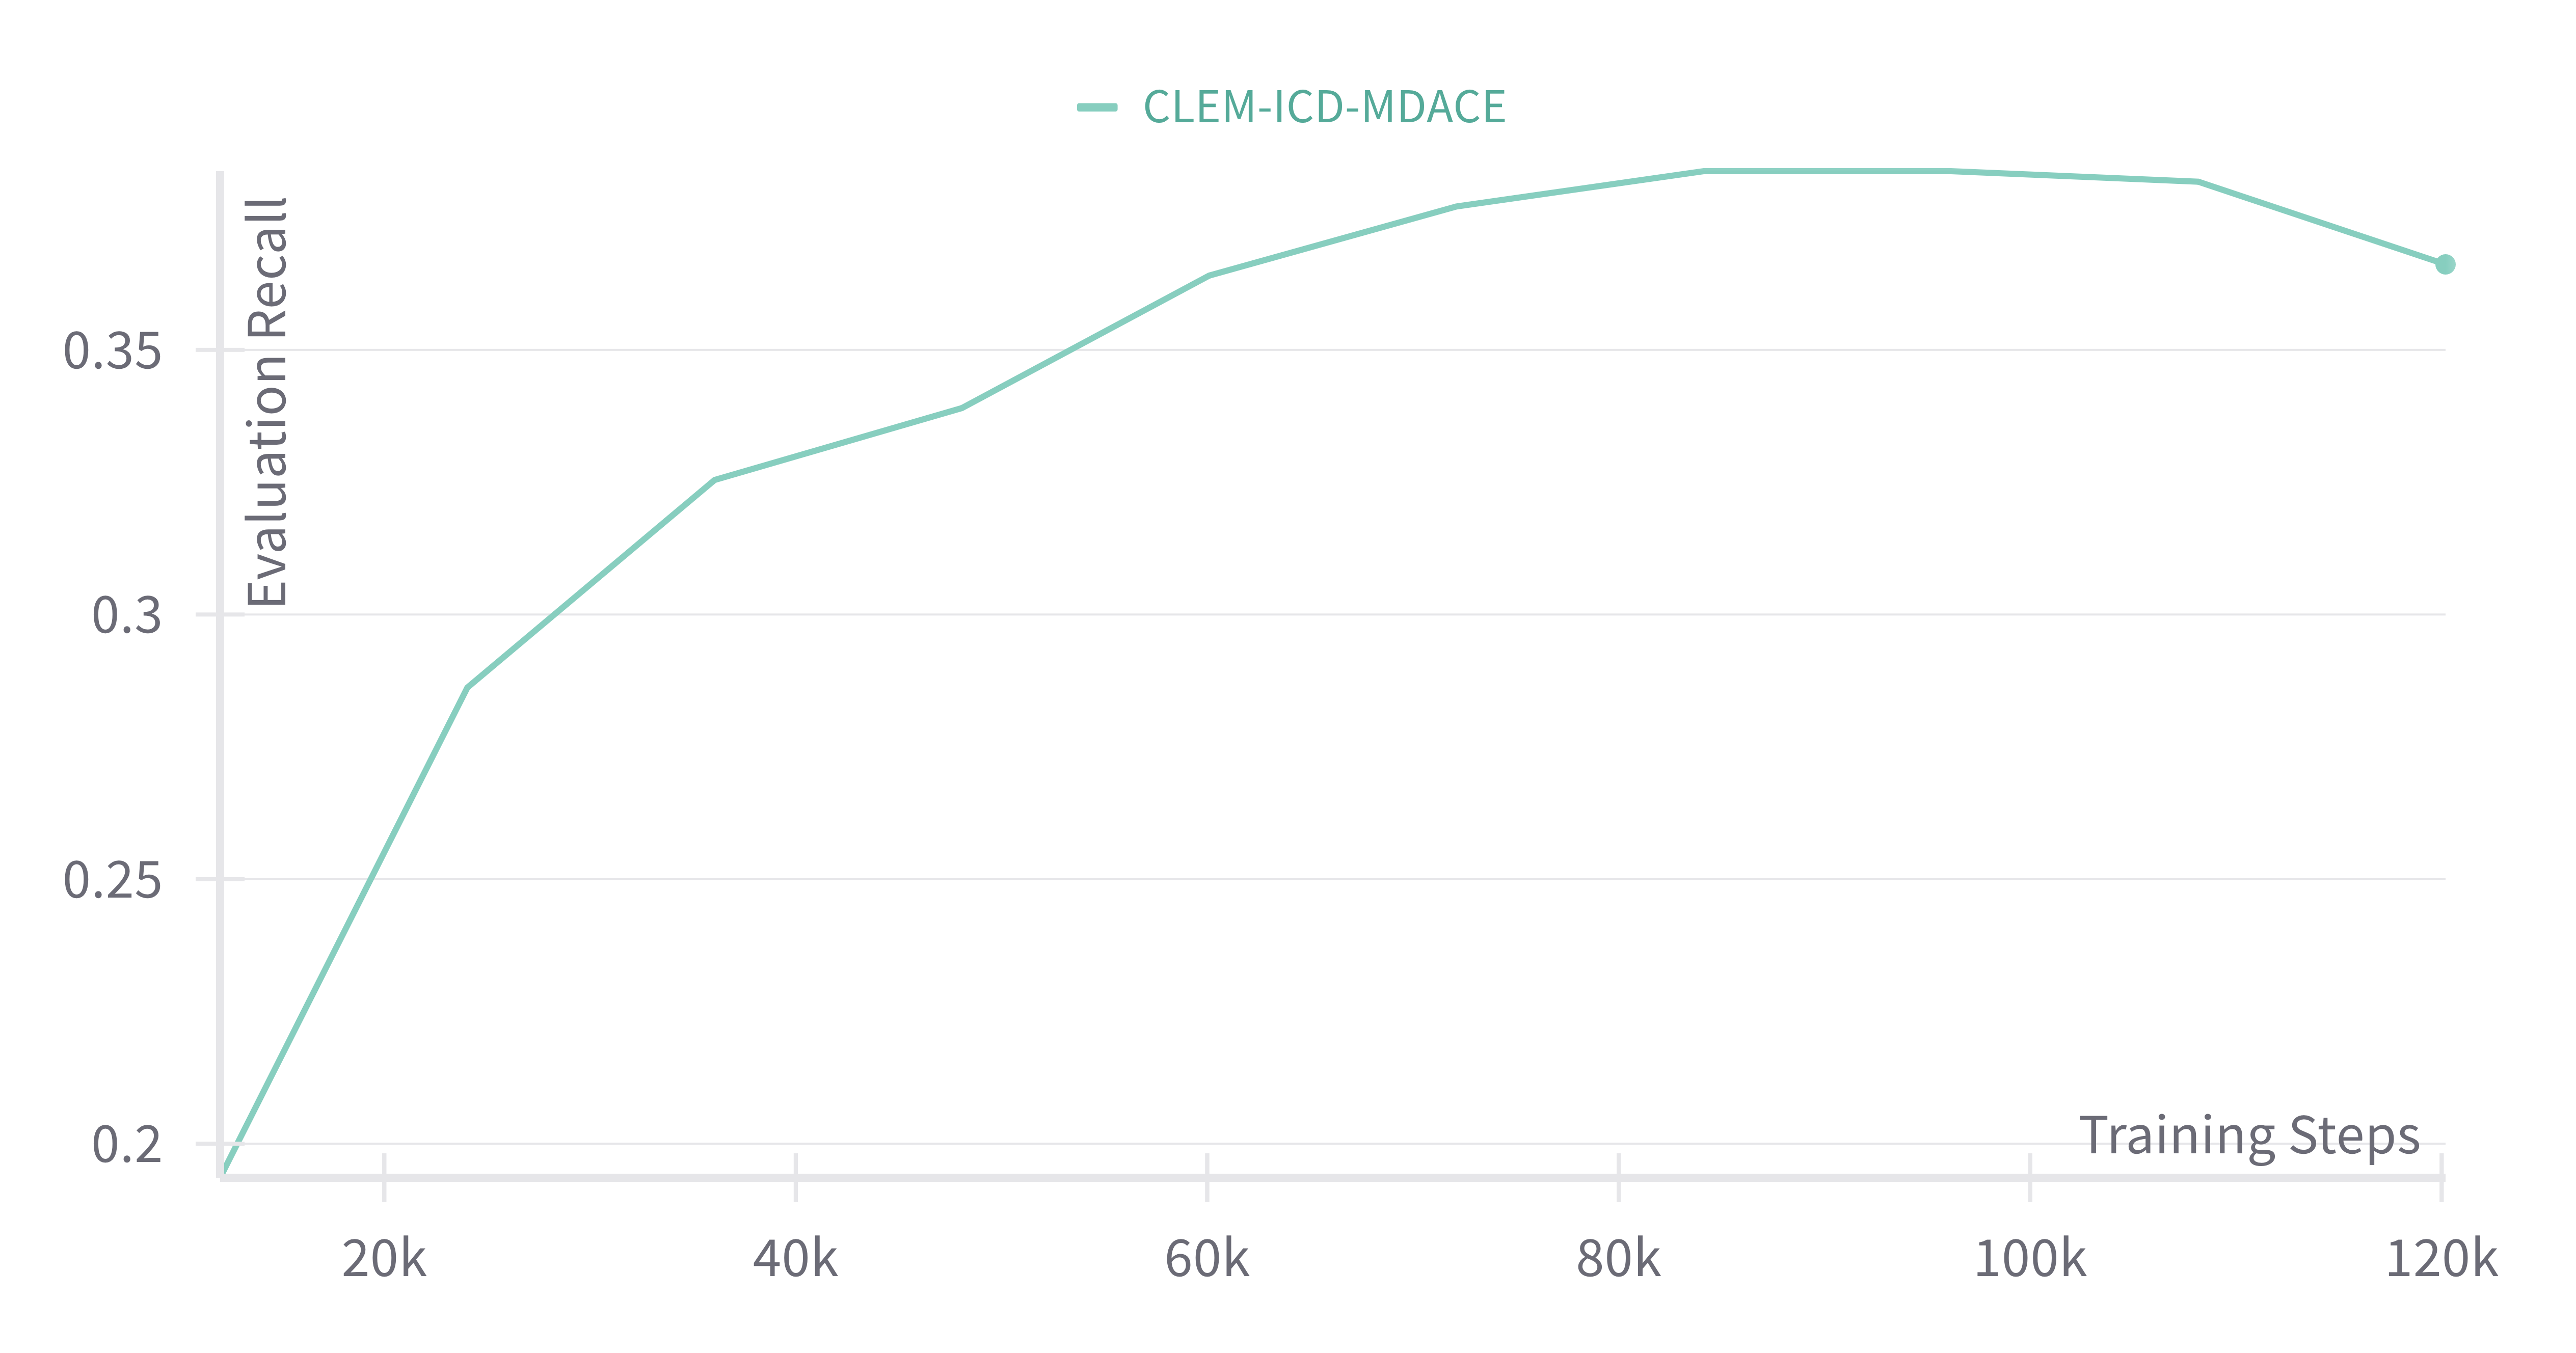
\includegraphics[keepaspectratio]{learning_curve_recall_mdace.png}}

}

\subcaption{\label{fig-recall-mdace}Evaluation Recall (MDACE)}

\end{minipage}%
%
\begin{minipage}{0.50\linewidth}

\centering{

\pandocbounded{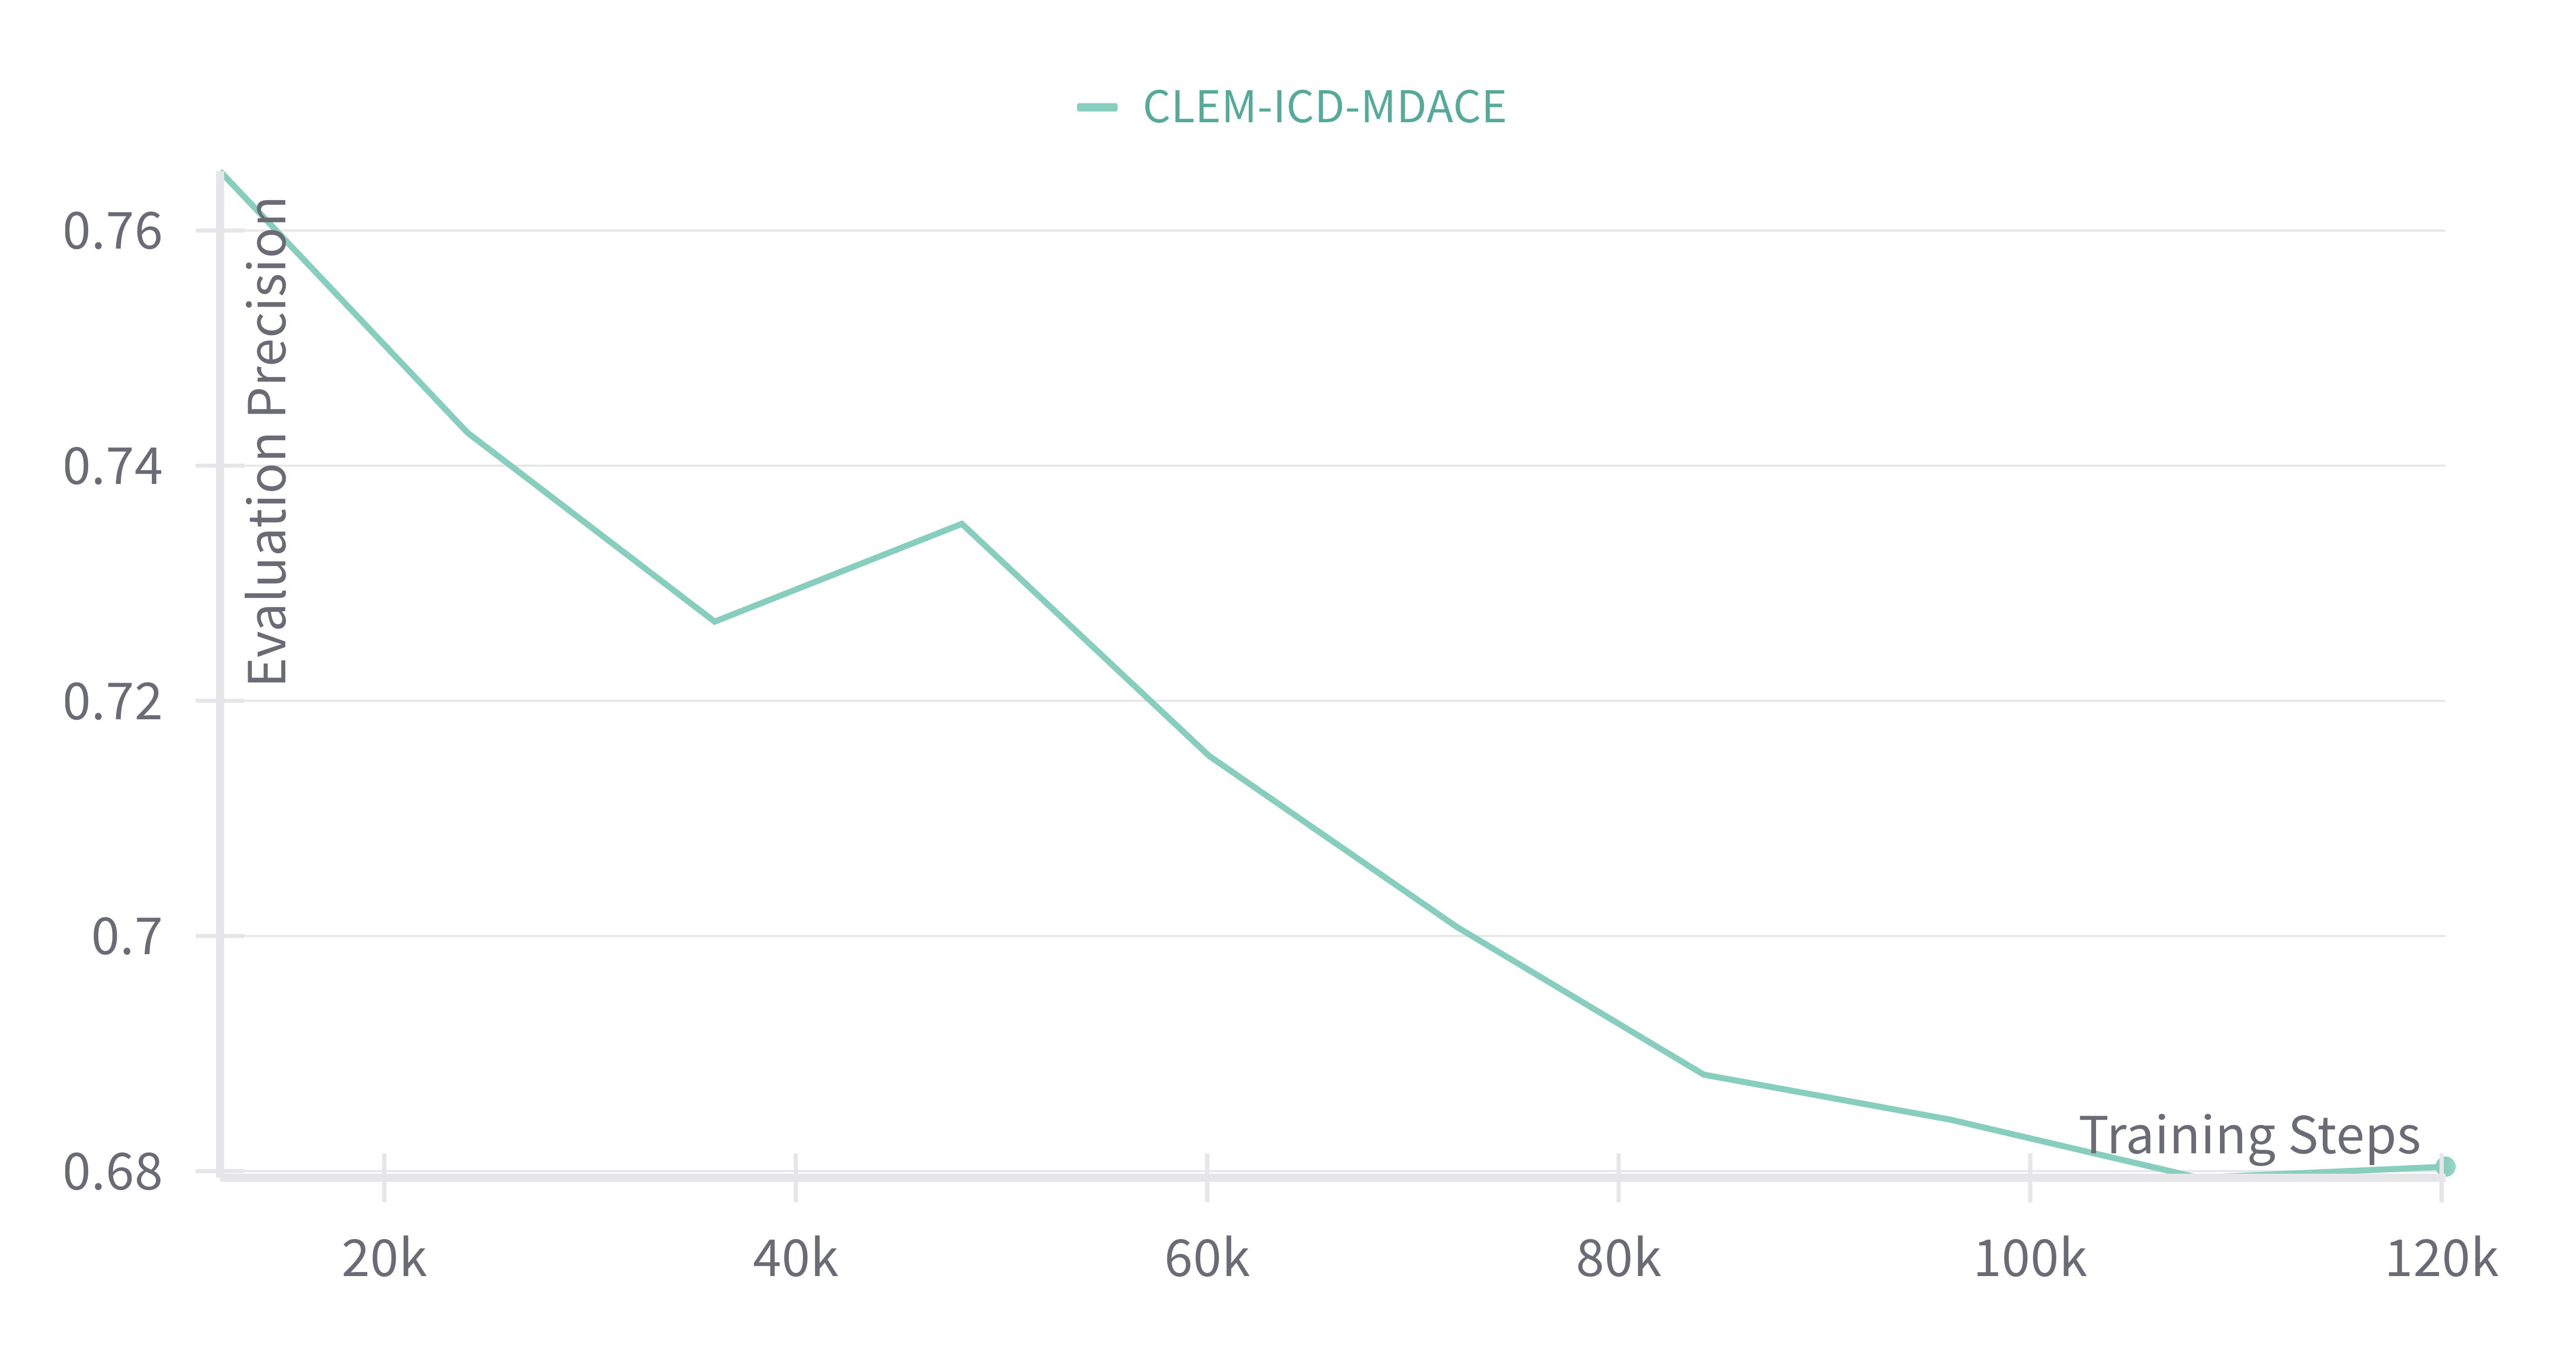
\includegraphics[keepaspectratio]{learning_curve_precision_mdace.png}}

}

\subcaption{\label{fig-precision-mdace}Evaluation Precision (MDACE)}

\end{minipage}%
\newline
\begin{minipage}{0.50\linewidth}

\centering{

\pandocbounded{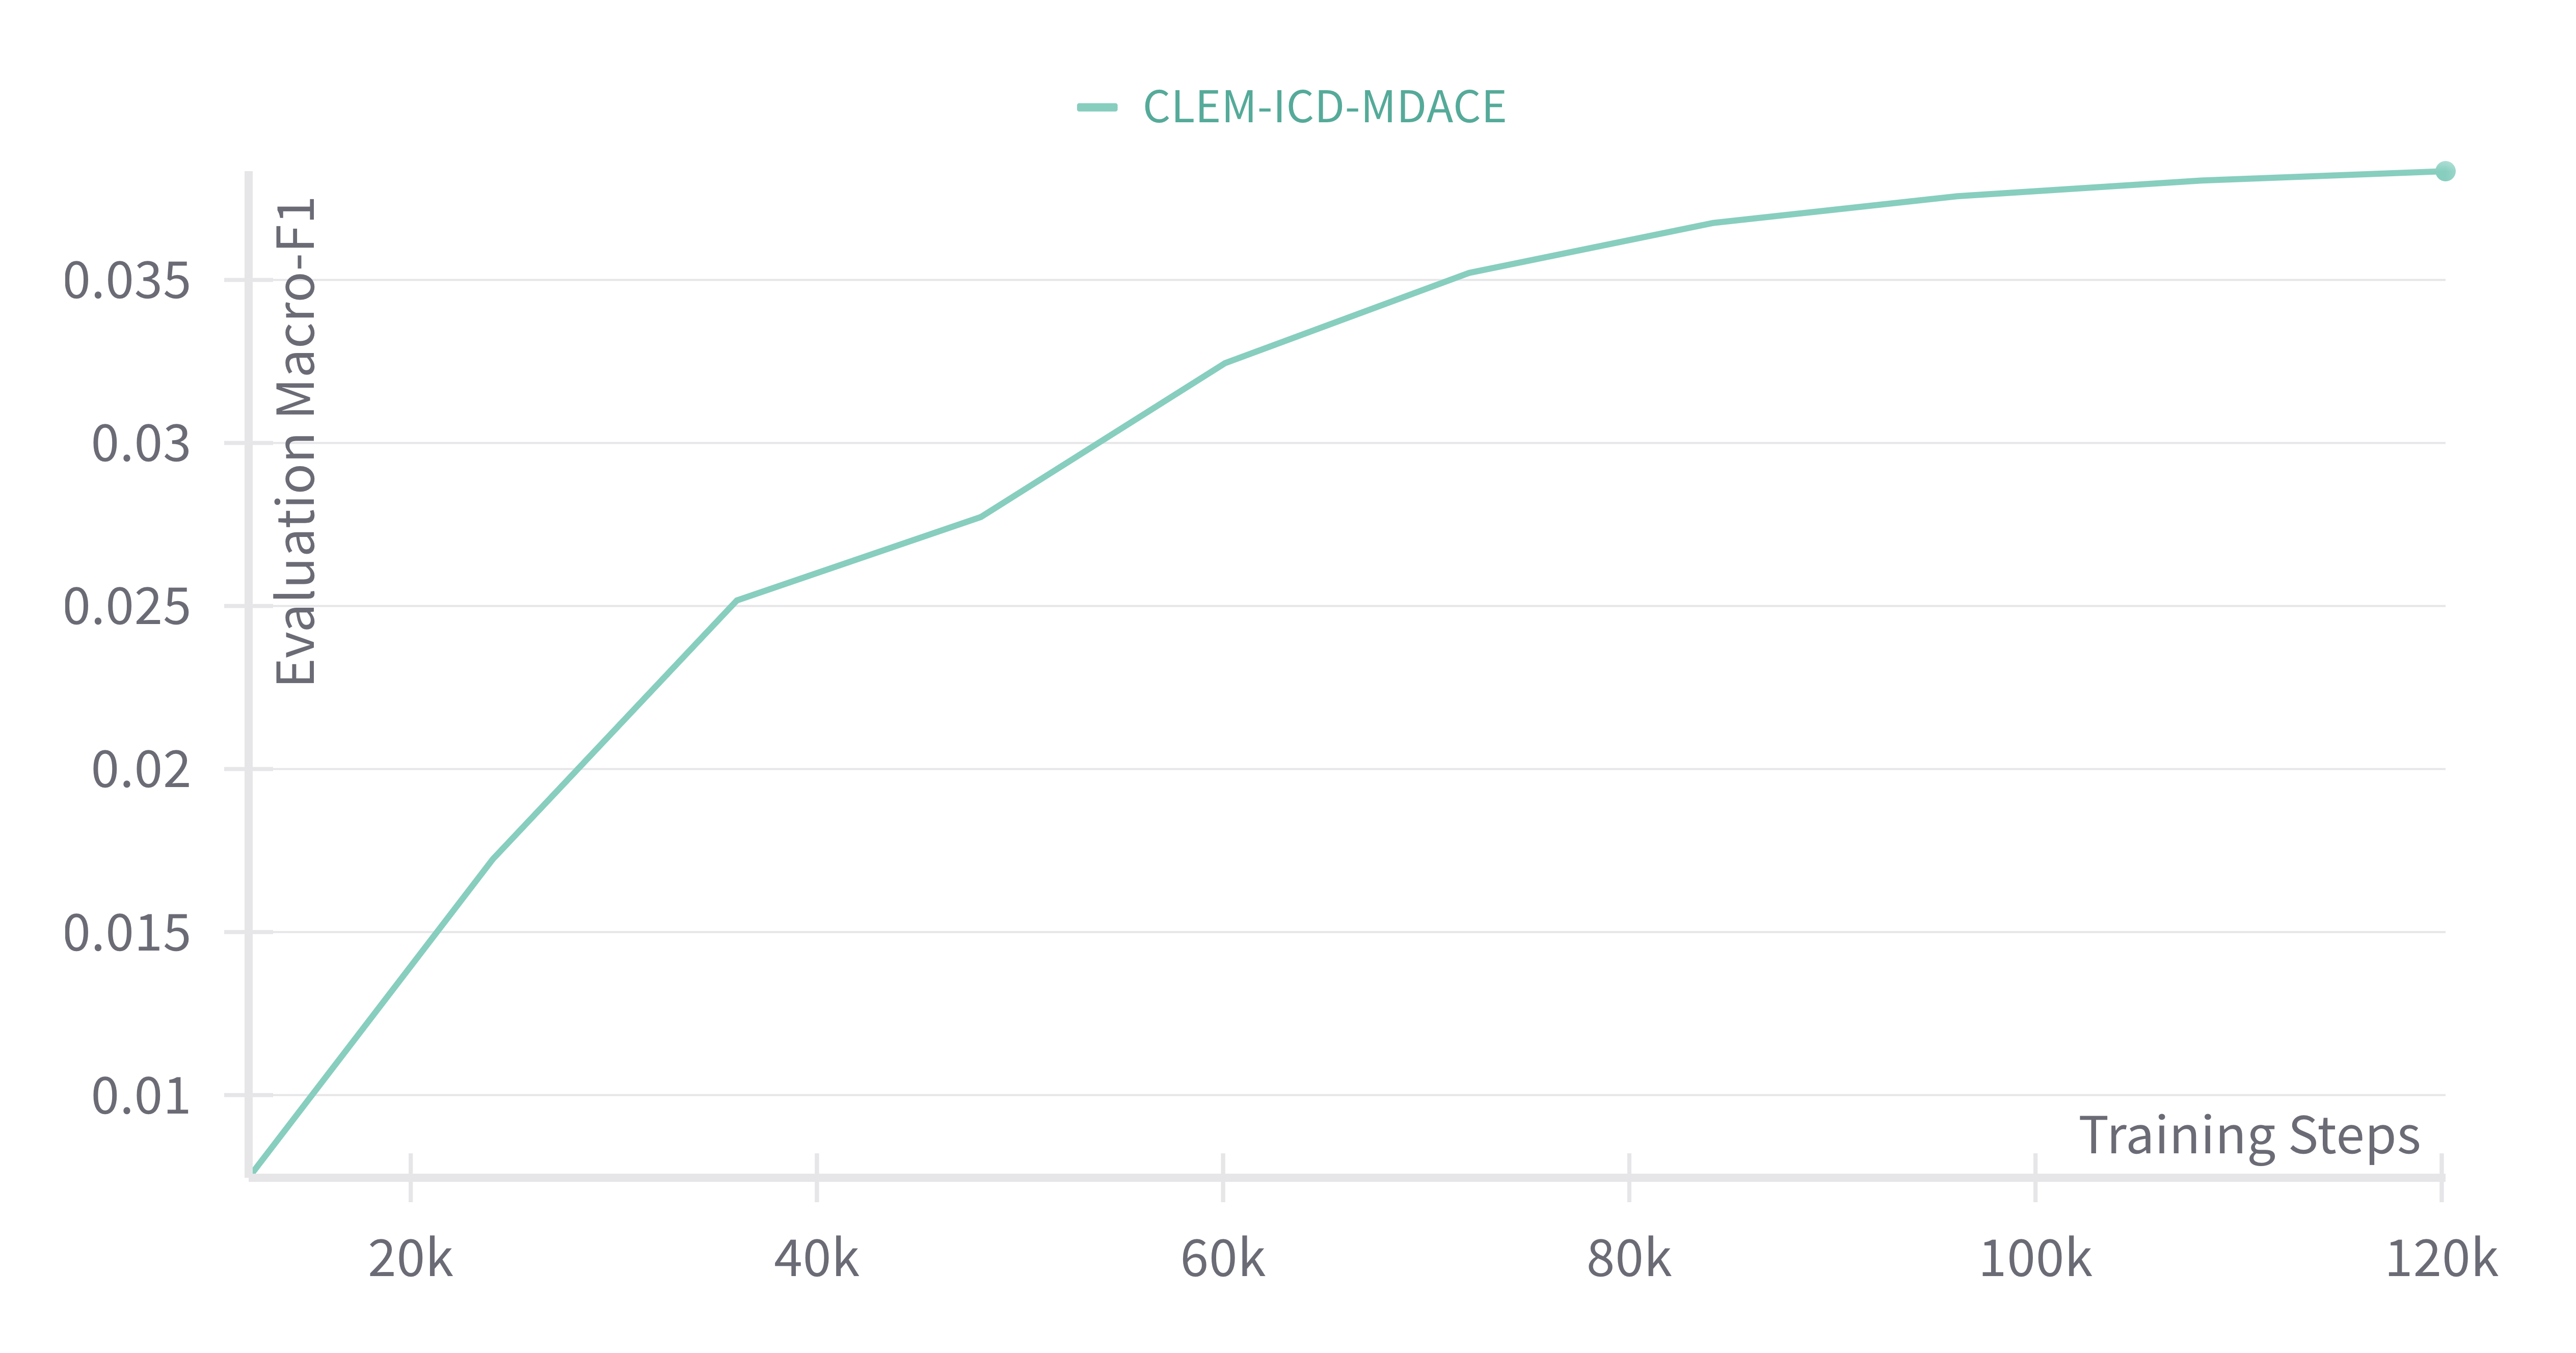
\includegraphics[keepaspectratio]{learning_curve_macro_f1_mdace.png}}

}

\subcaption{\label{fig-macro-f1-mdace}Evaluation Macro-F1 Score (MDACE)}

\end{minipage}%
%
\begin{minipage}{0.50\linewidth}

\centering{

\pandocbounded{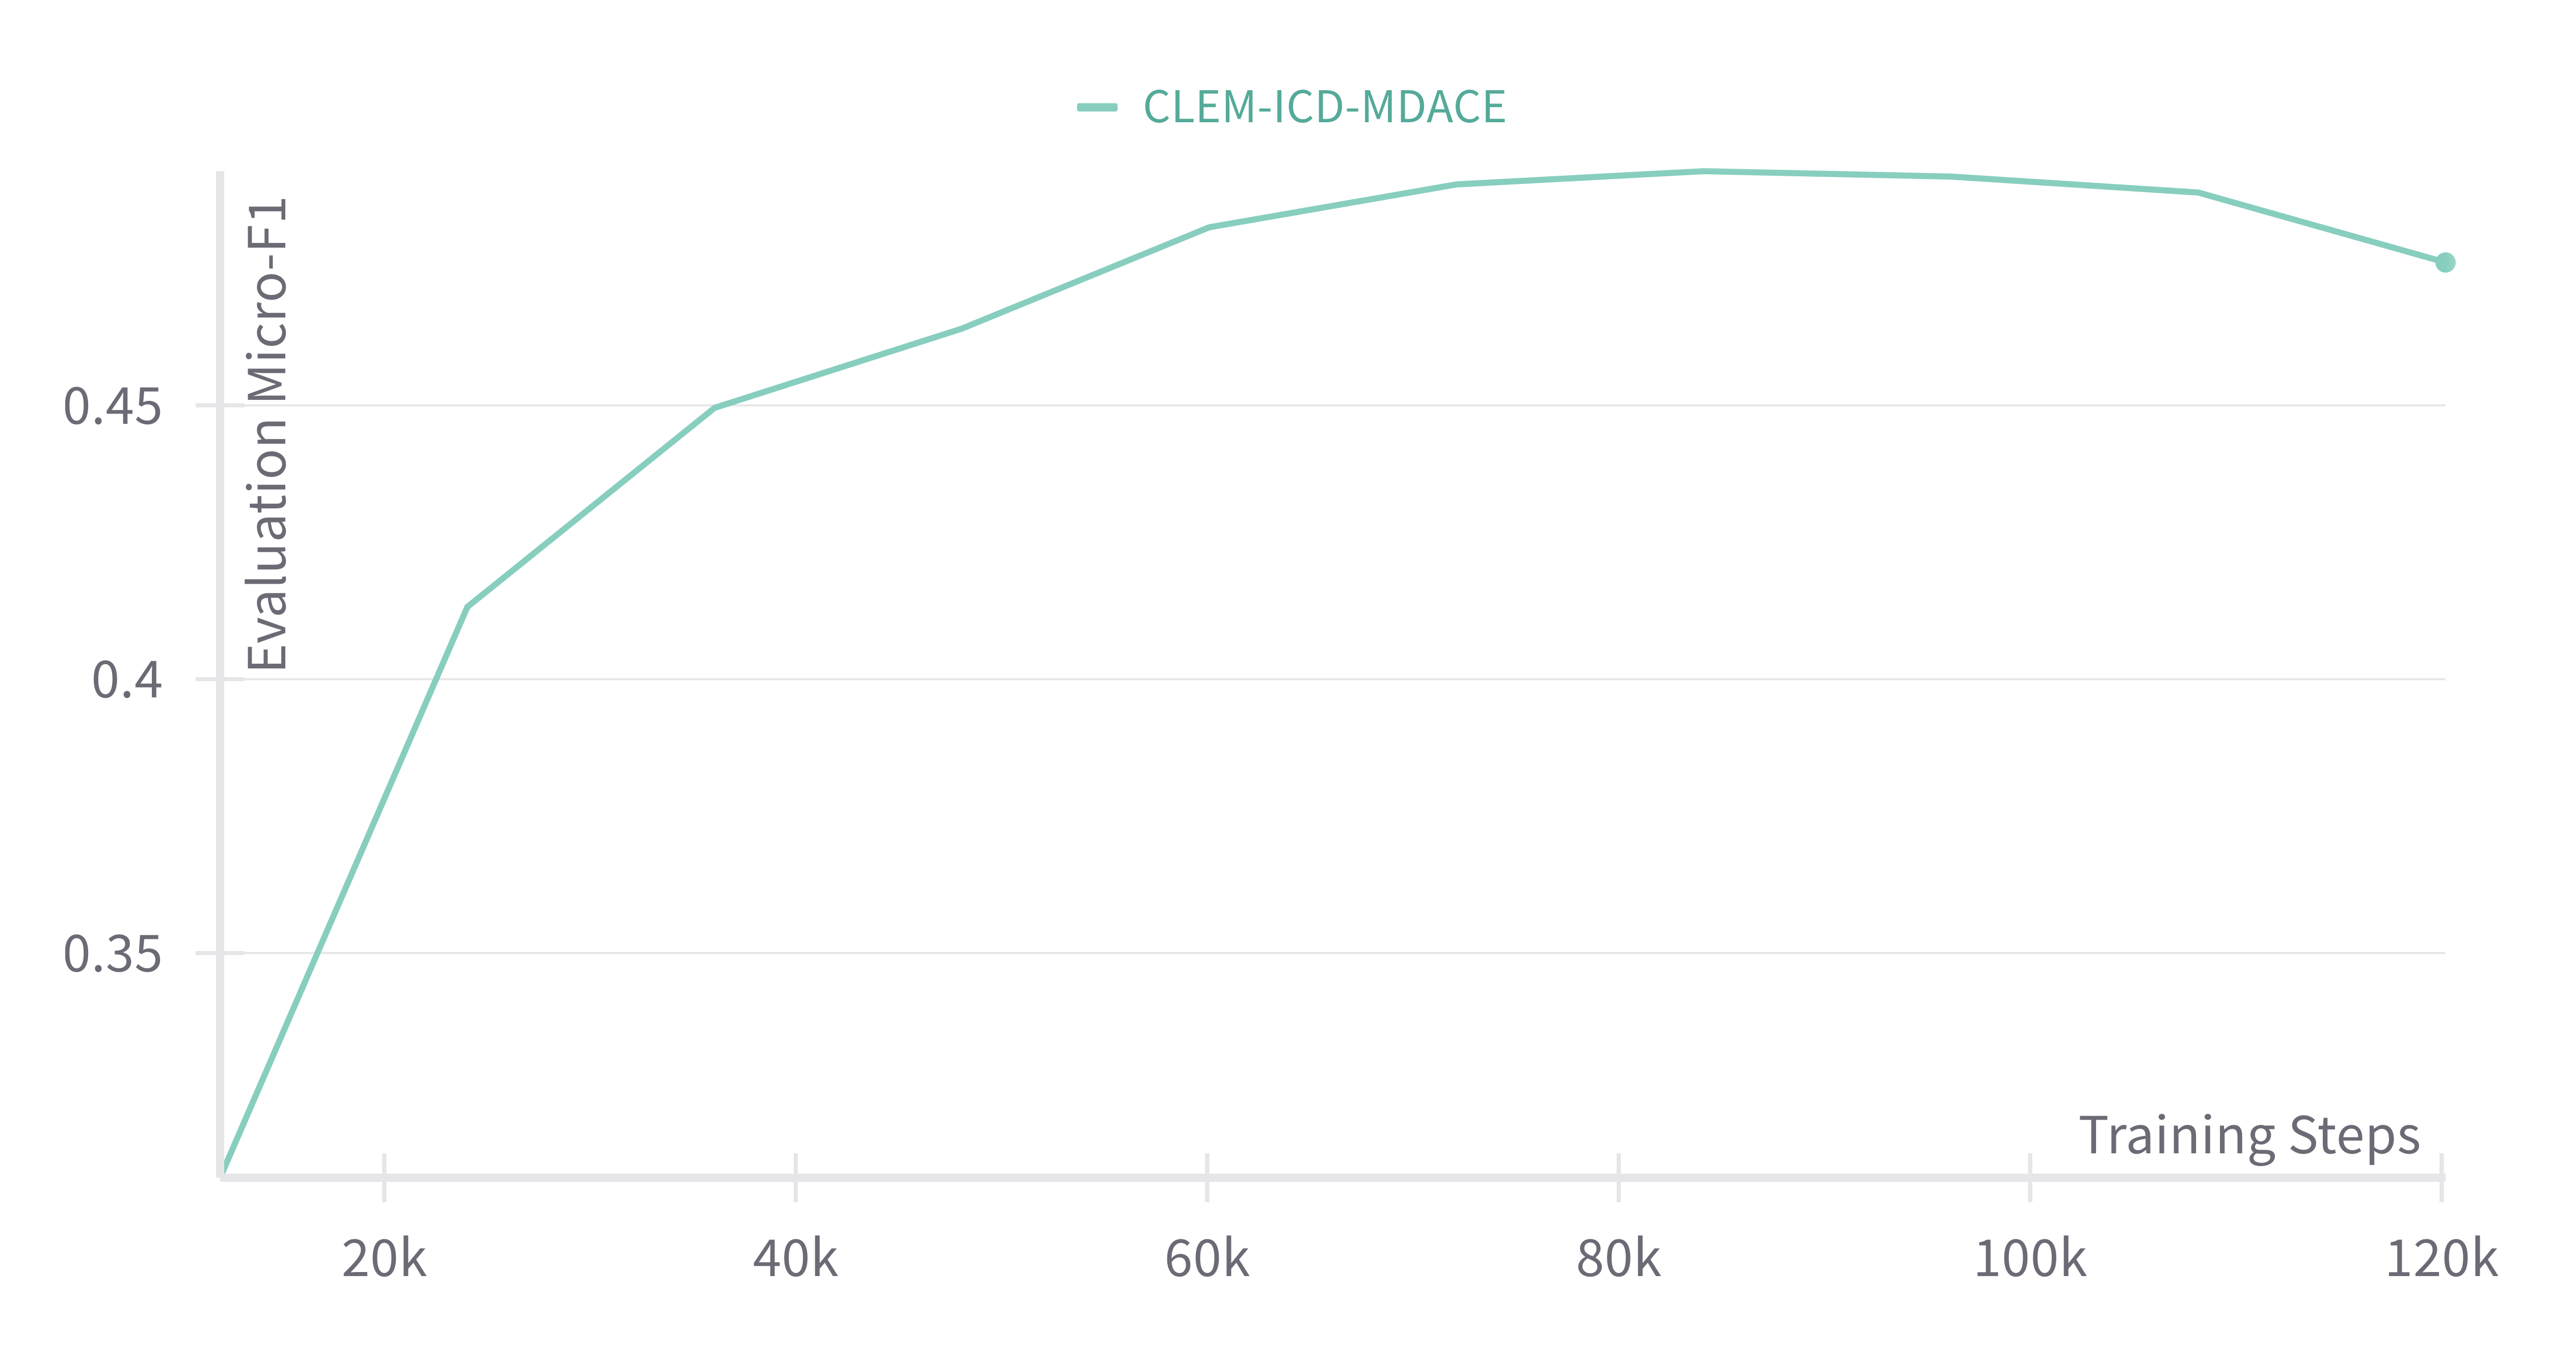
\includegraphics[keepaspectratio]{learning_curve_micro_f1_mdace.png}}

}

\subcaption{\label{fig-micro-f1-mdace}Evaluation Micro-F1 Score (MDACE)}

\end{minipage}%

\caption{\label{fig-learning-curves-mdace}Learning curves for CLEM-ICD
trained on MIMIC-III Inpatient Discharge Summaries (MDACE splits) for 10
epochs.}

\end{figure}%

\begin{figure}

\begin{minipage}{0.50\linewidth}

\centering{

\pandocbounded{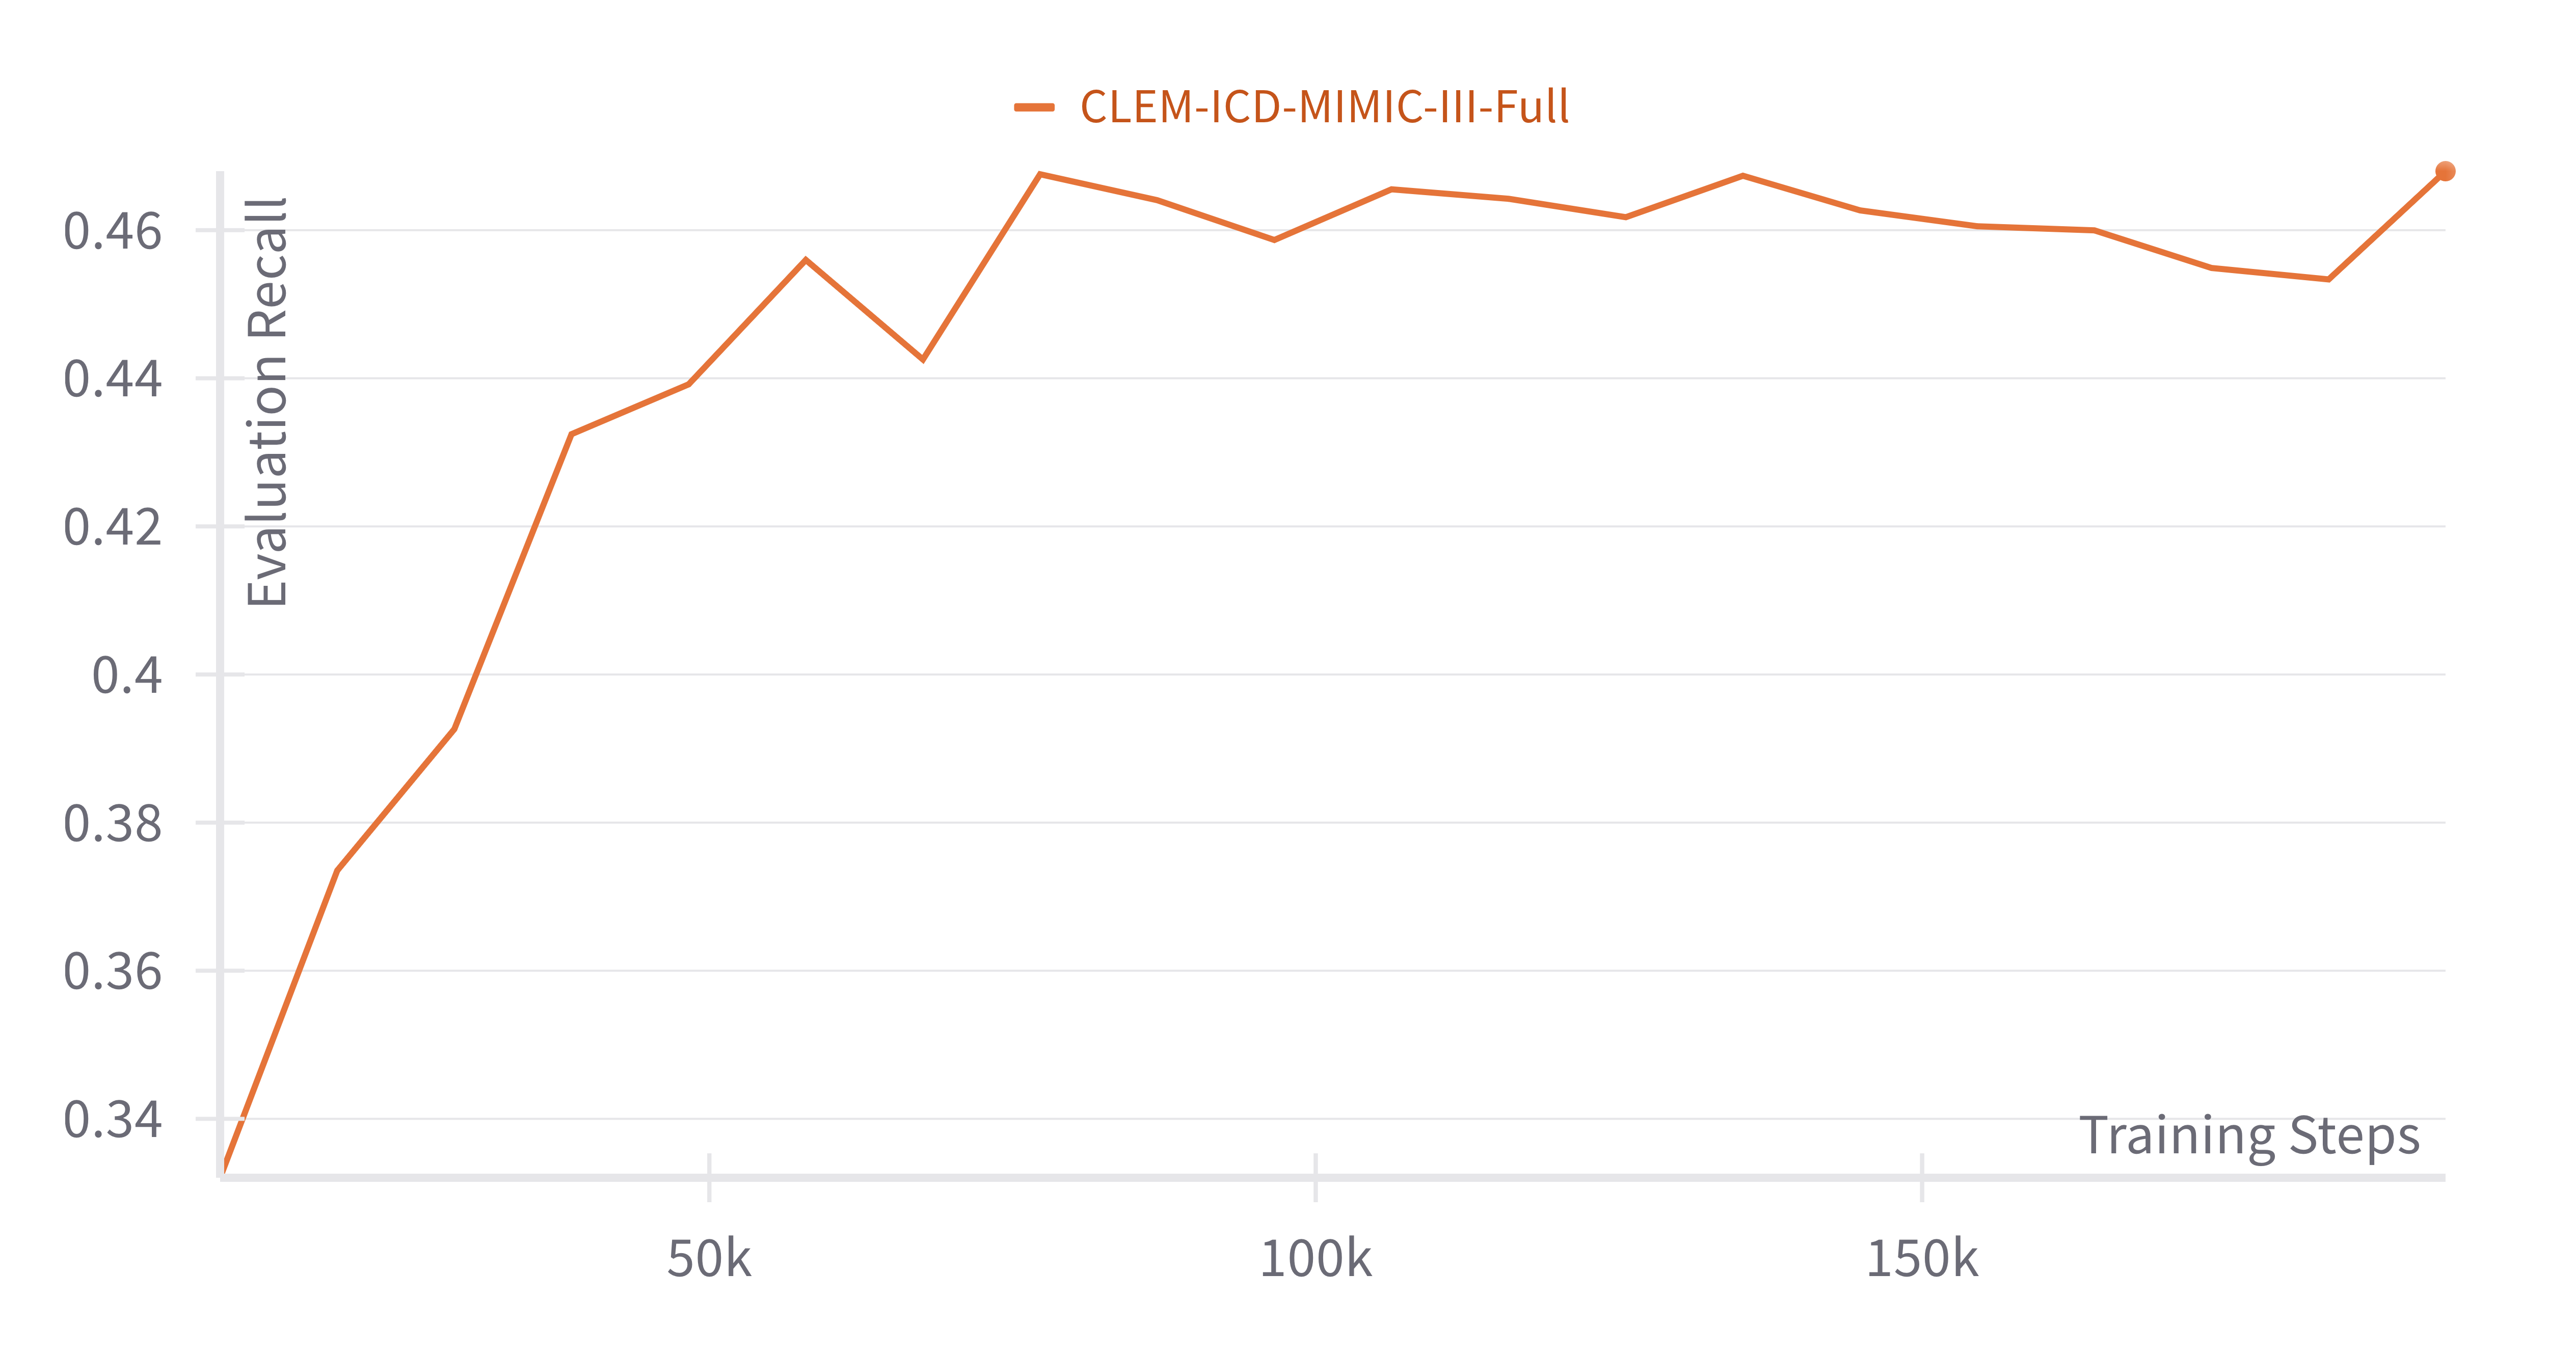
\includegraphics[keepaspectratio]{learning_curve_recall_full.png}}

}

\subcaption{\label{fig-recall-full}Evaluation Recall (MIMIC-III Full)}

\end{minipage}%
%
\begin{minipage}{0.50\linewidth}

\centering{

\pandocbounded{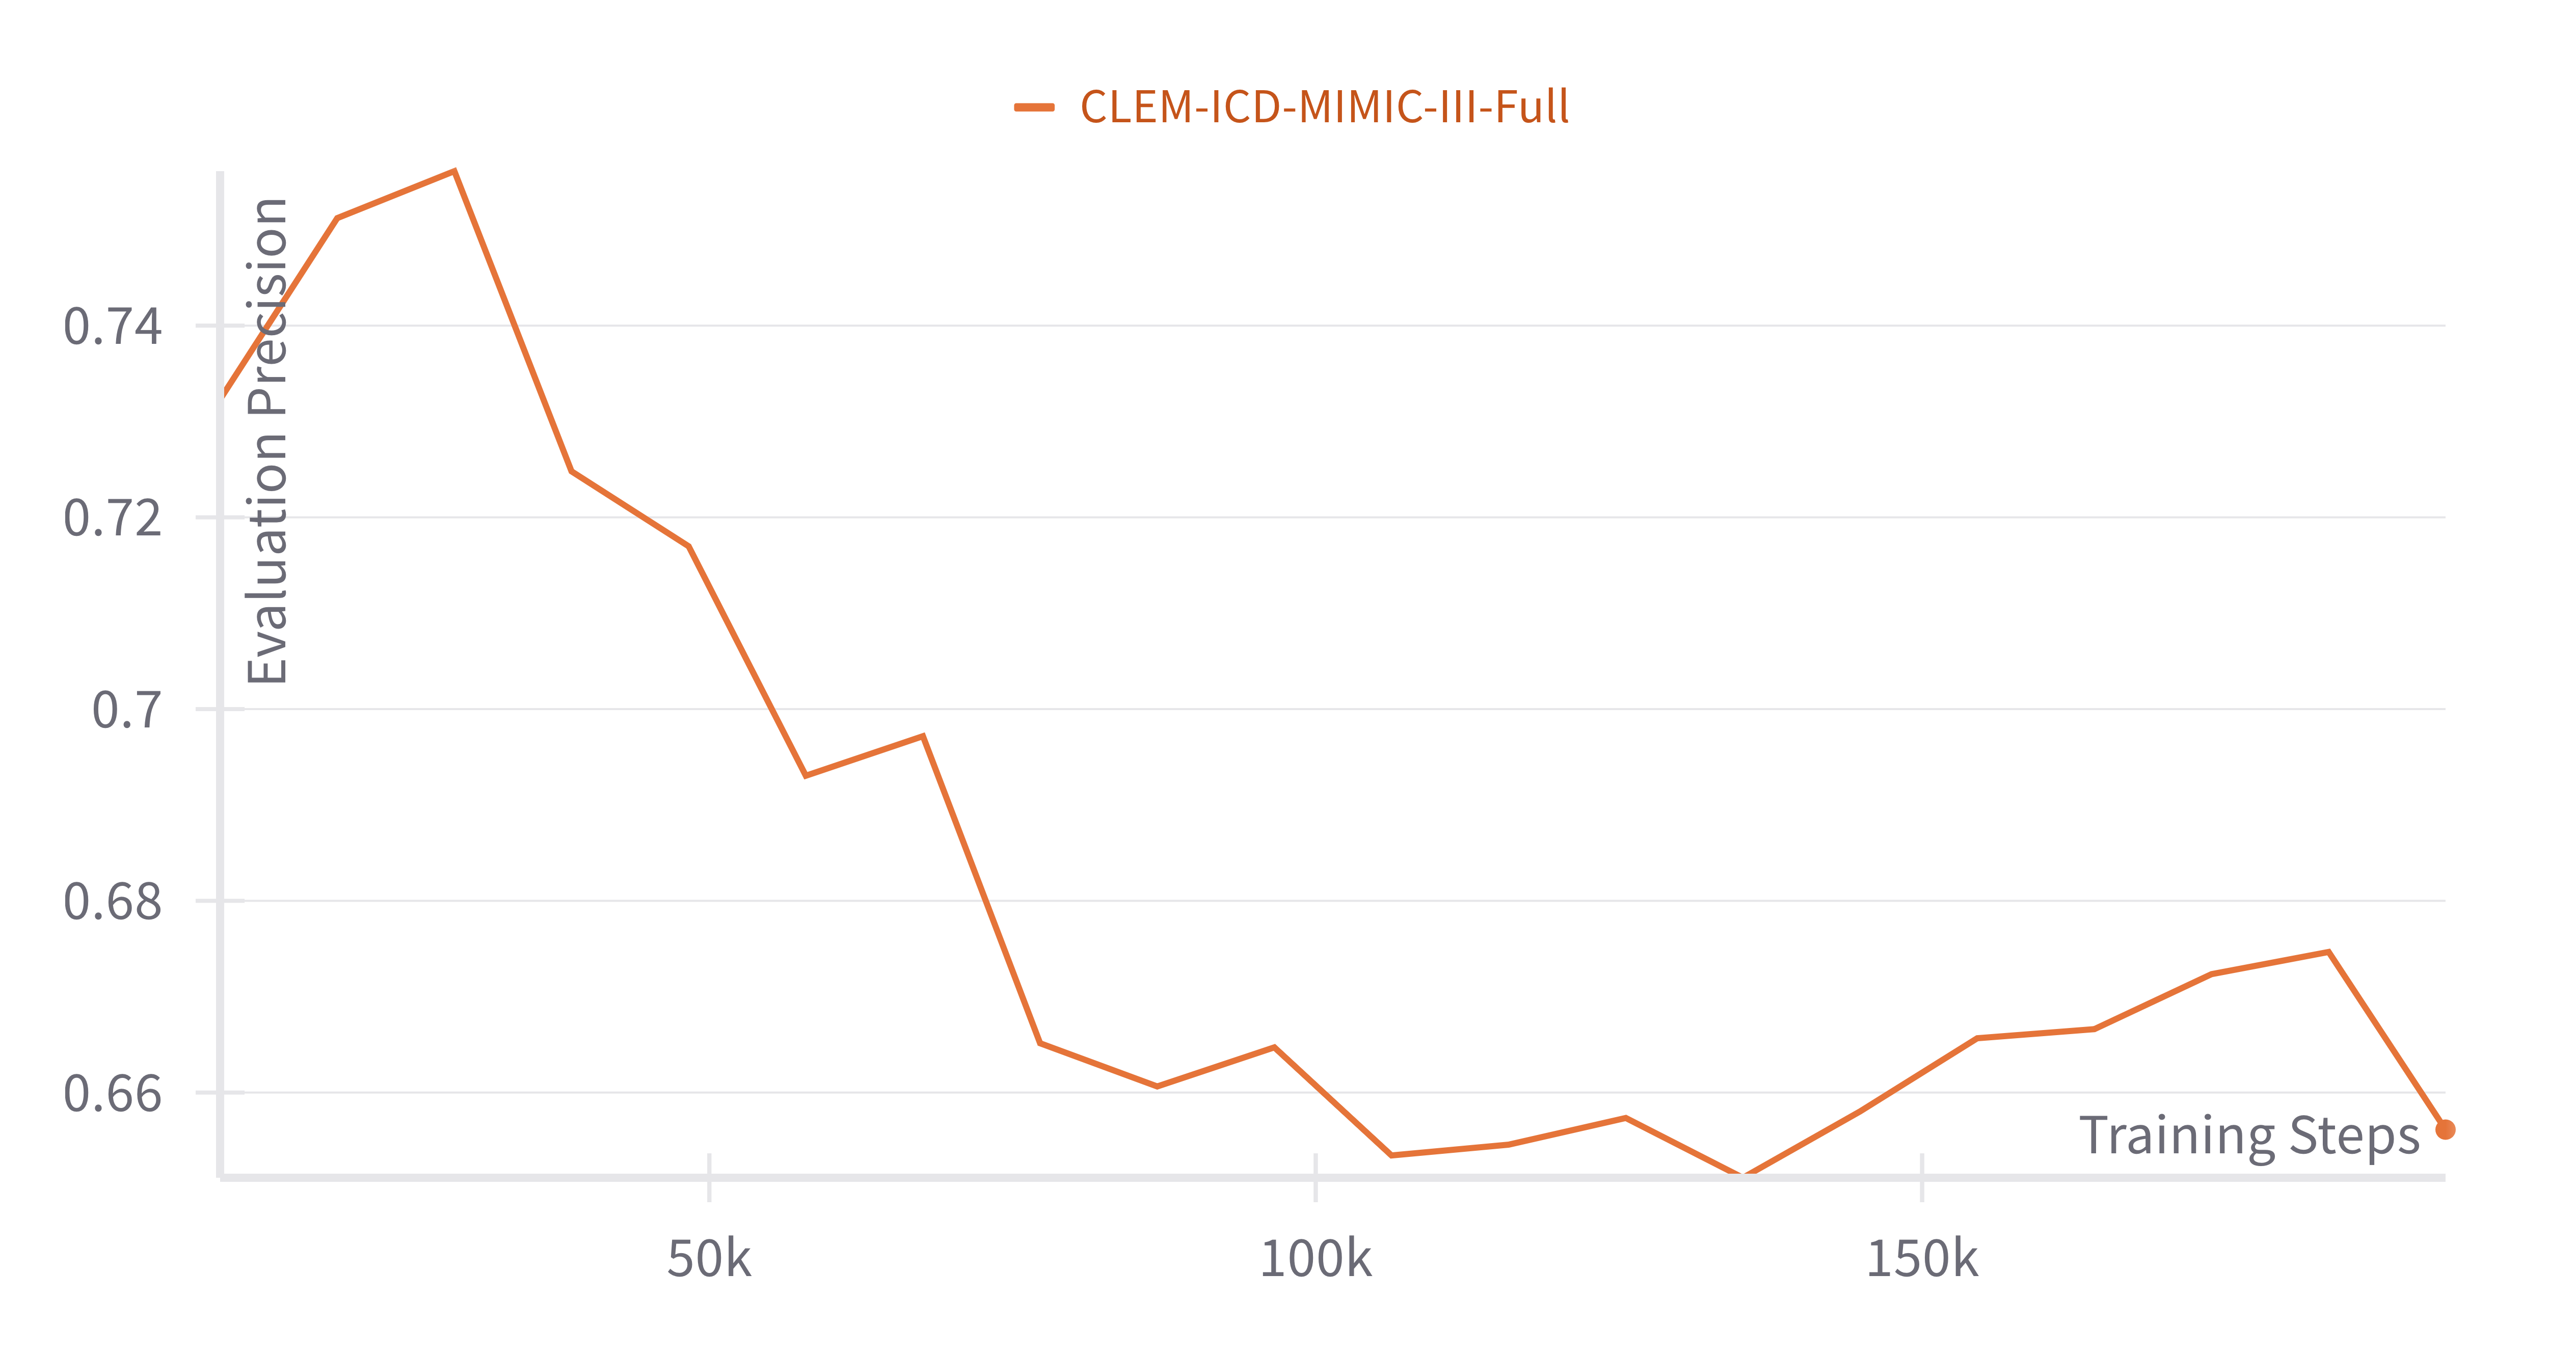
\includegraphics[keepaspectratio]{learning_curve_precision_full.png}}

}

\subcaption{\label{fig-precision-full}Evaluation Precision (MIMIC-III
Full)}

\end{minipage}%
\newline
\begin{minipage}{0.50\linewidth}

\centering{

\pandocbounded{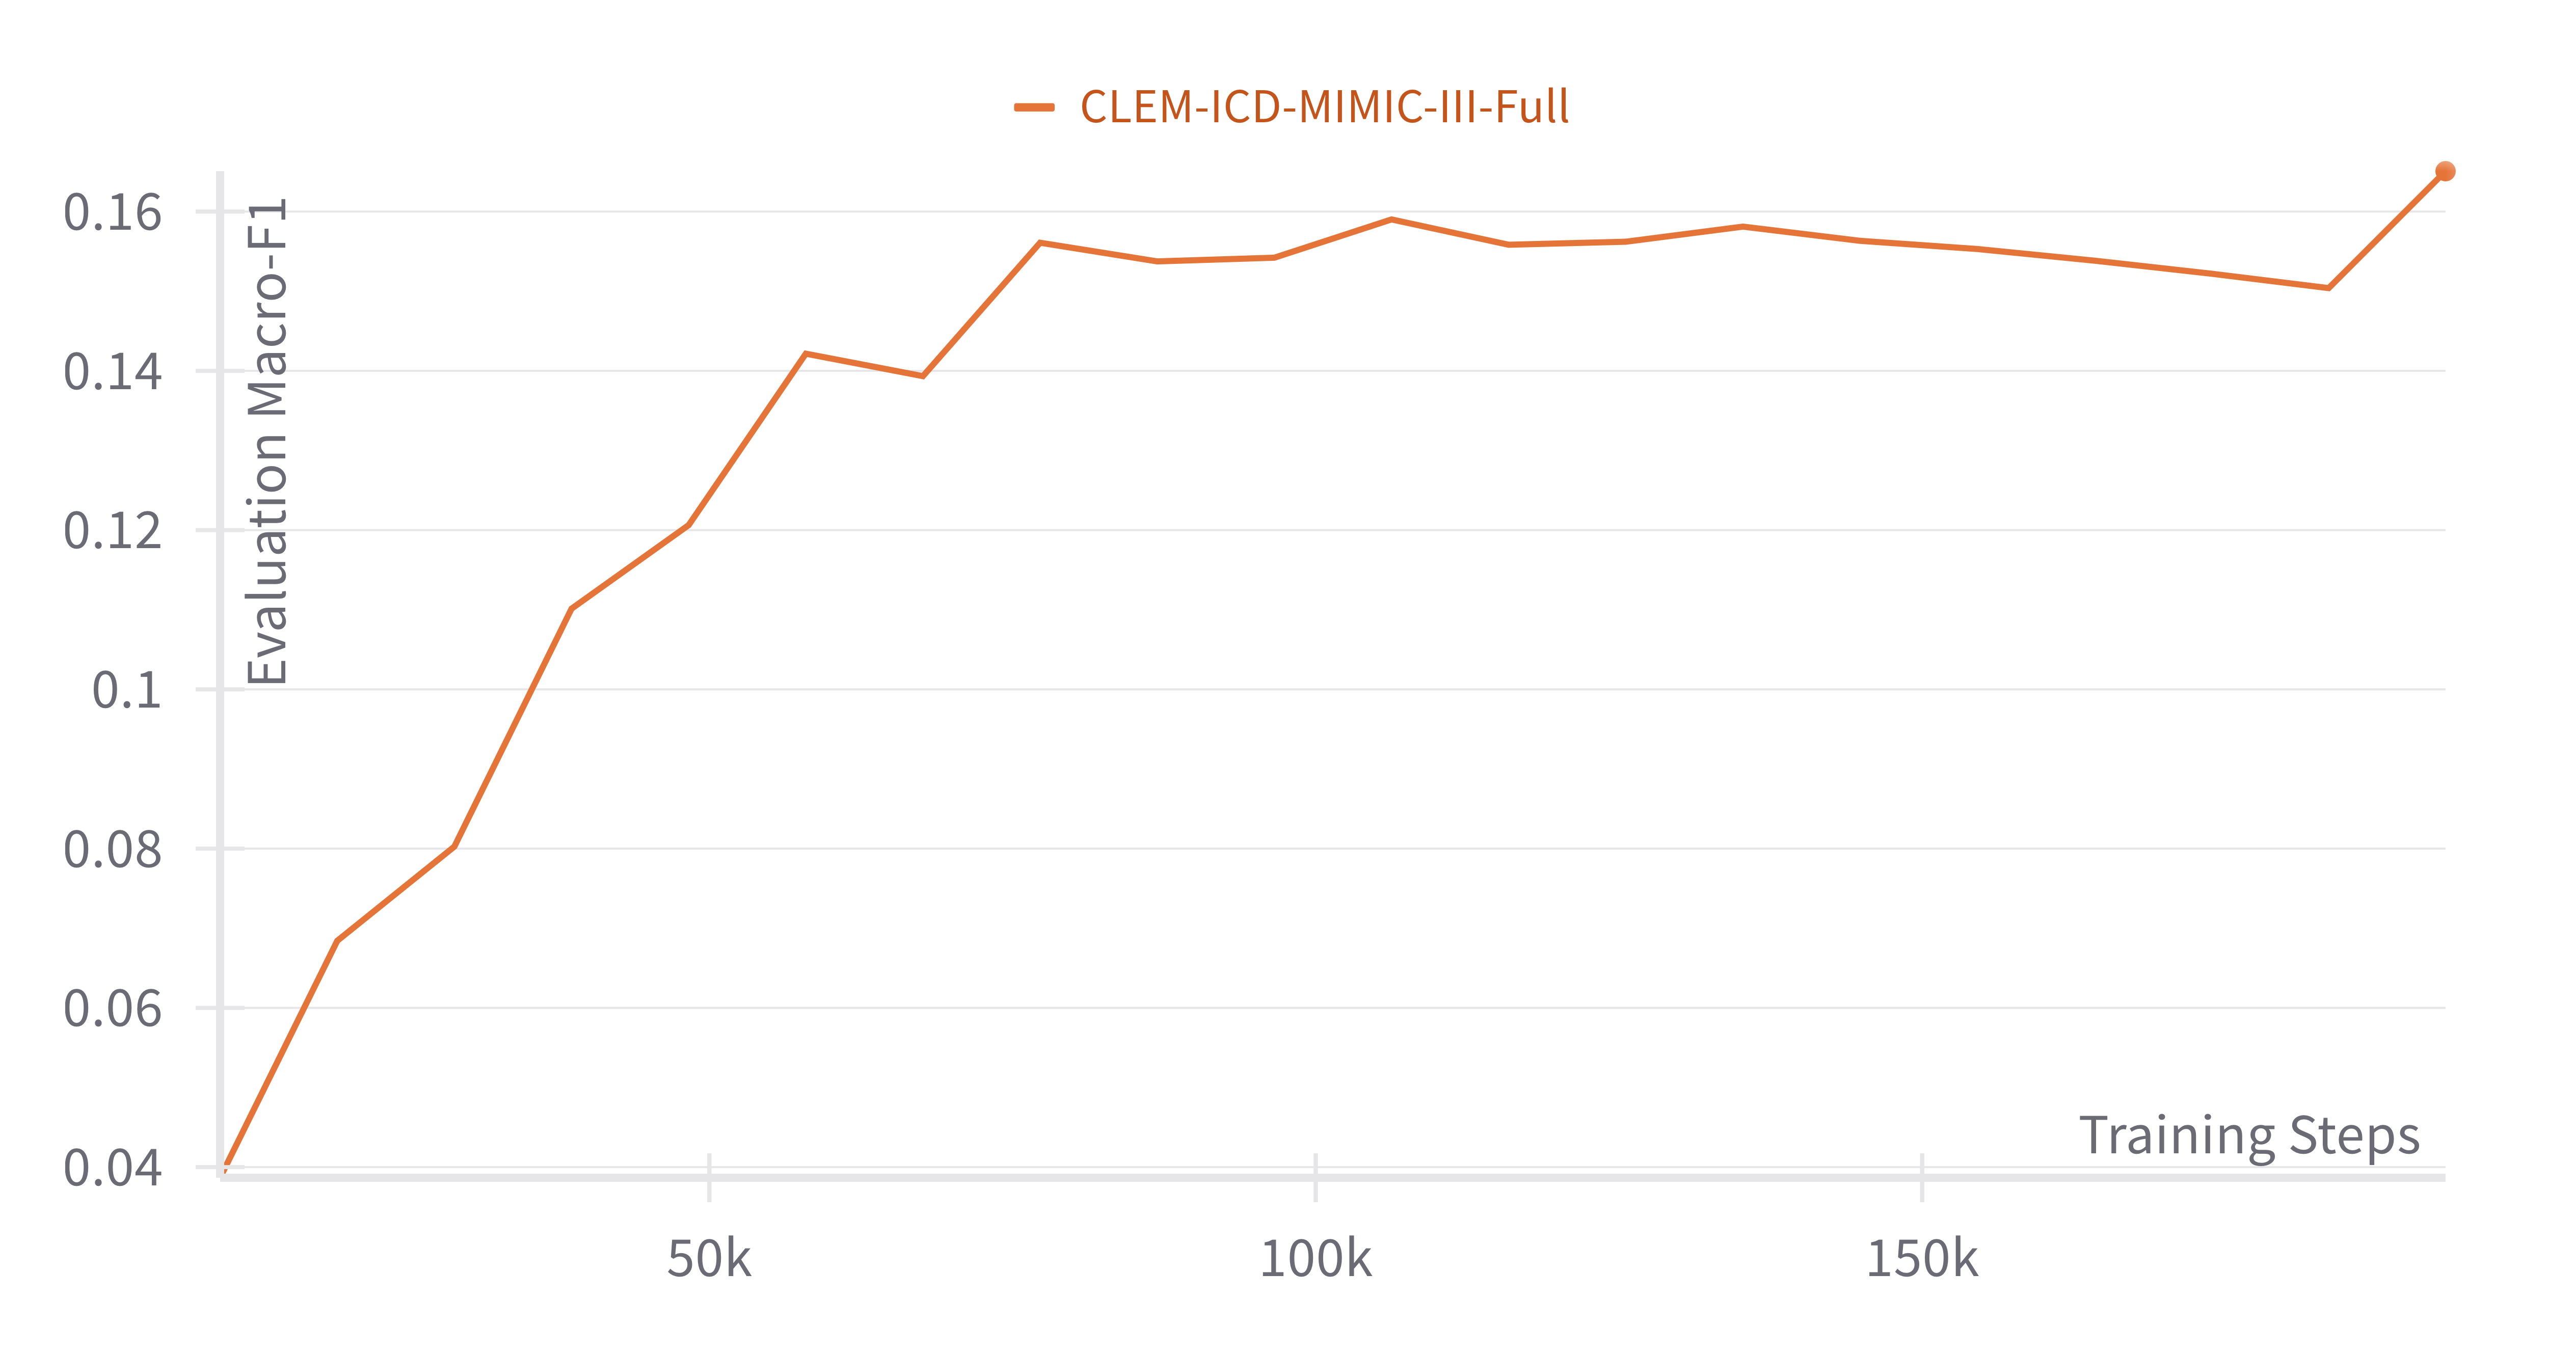
\includegraphics[keepaspectratio]{learning_curve_macro_f1_full.png}}

}

\subcaption{\label{fig-macro-f1-full}Evaluation Macro-F1 Score
(MIMIC-III Full)}

\end{minipage}%
%
\begin{minipage}{0.50\linewidth}

\centering{

\pandocbounded{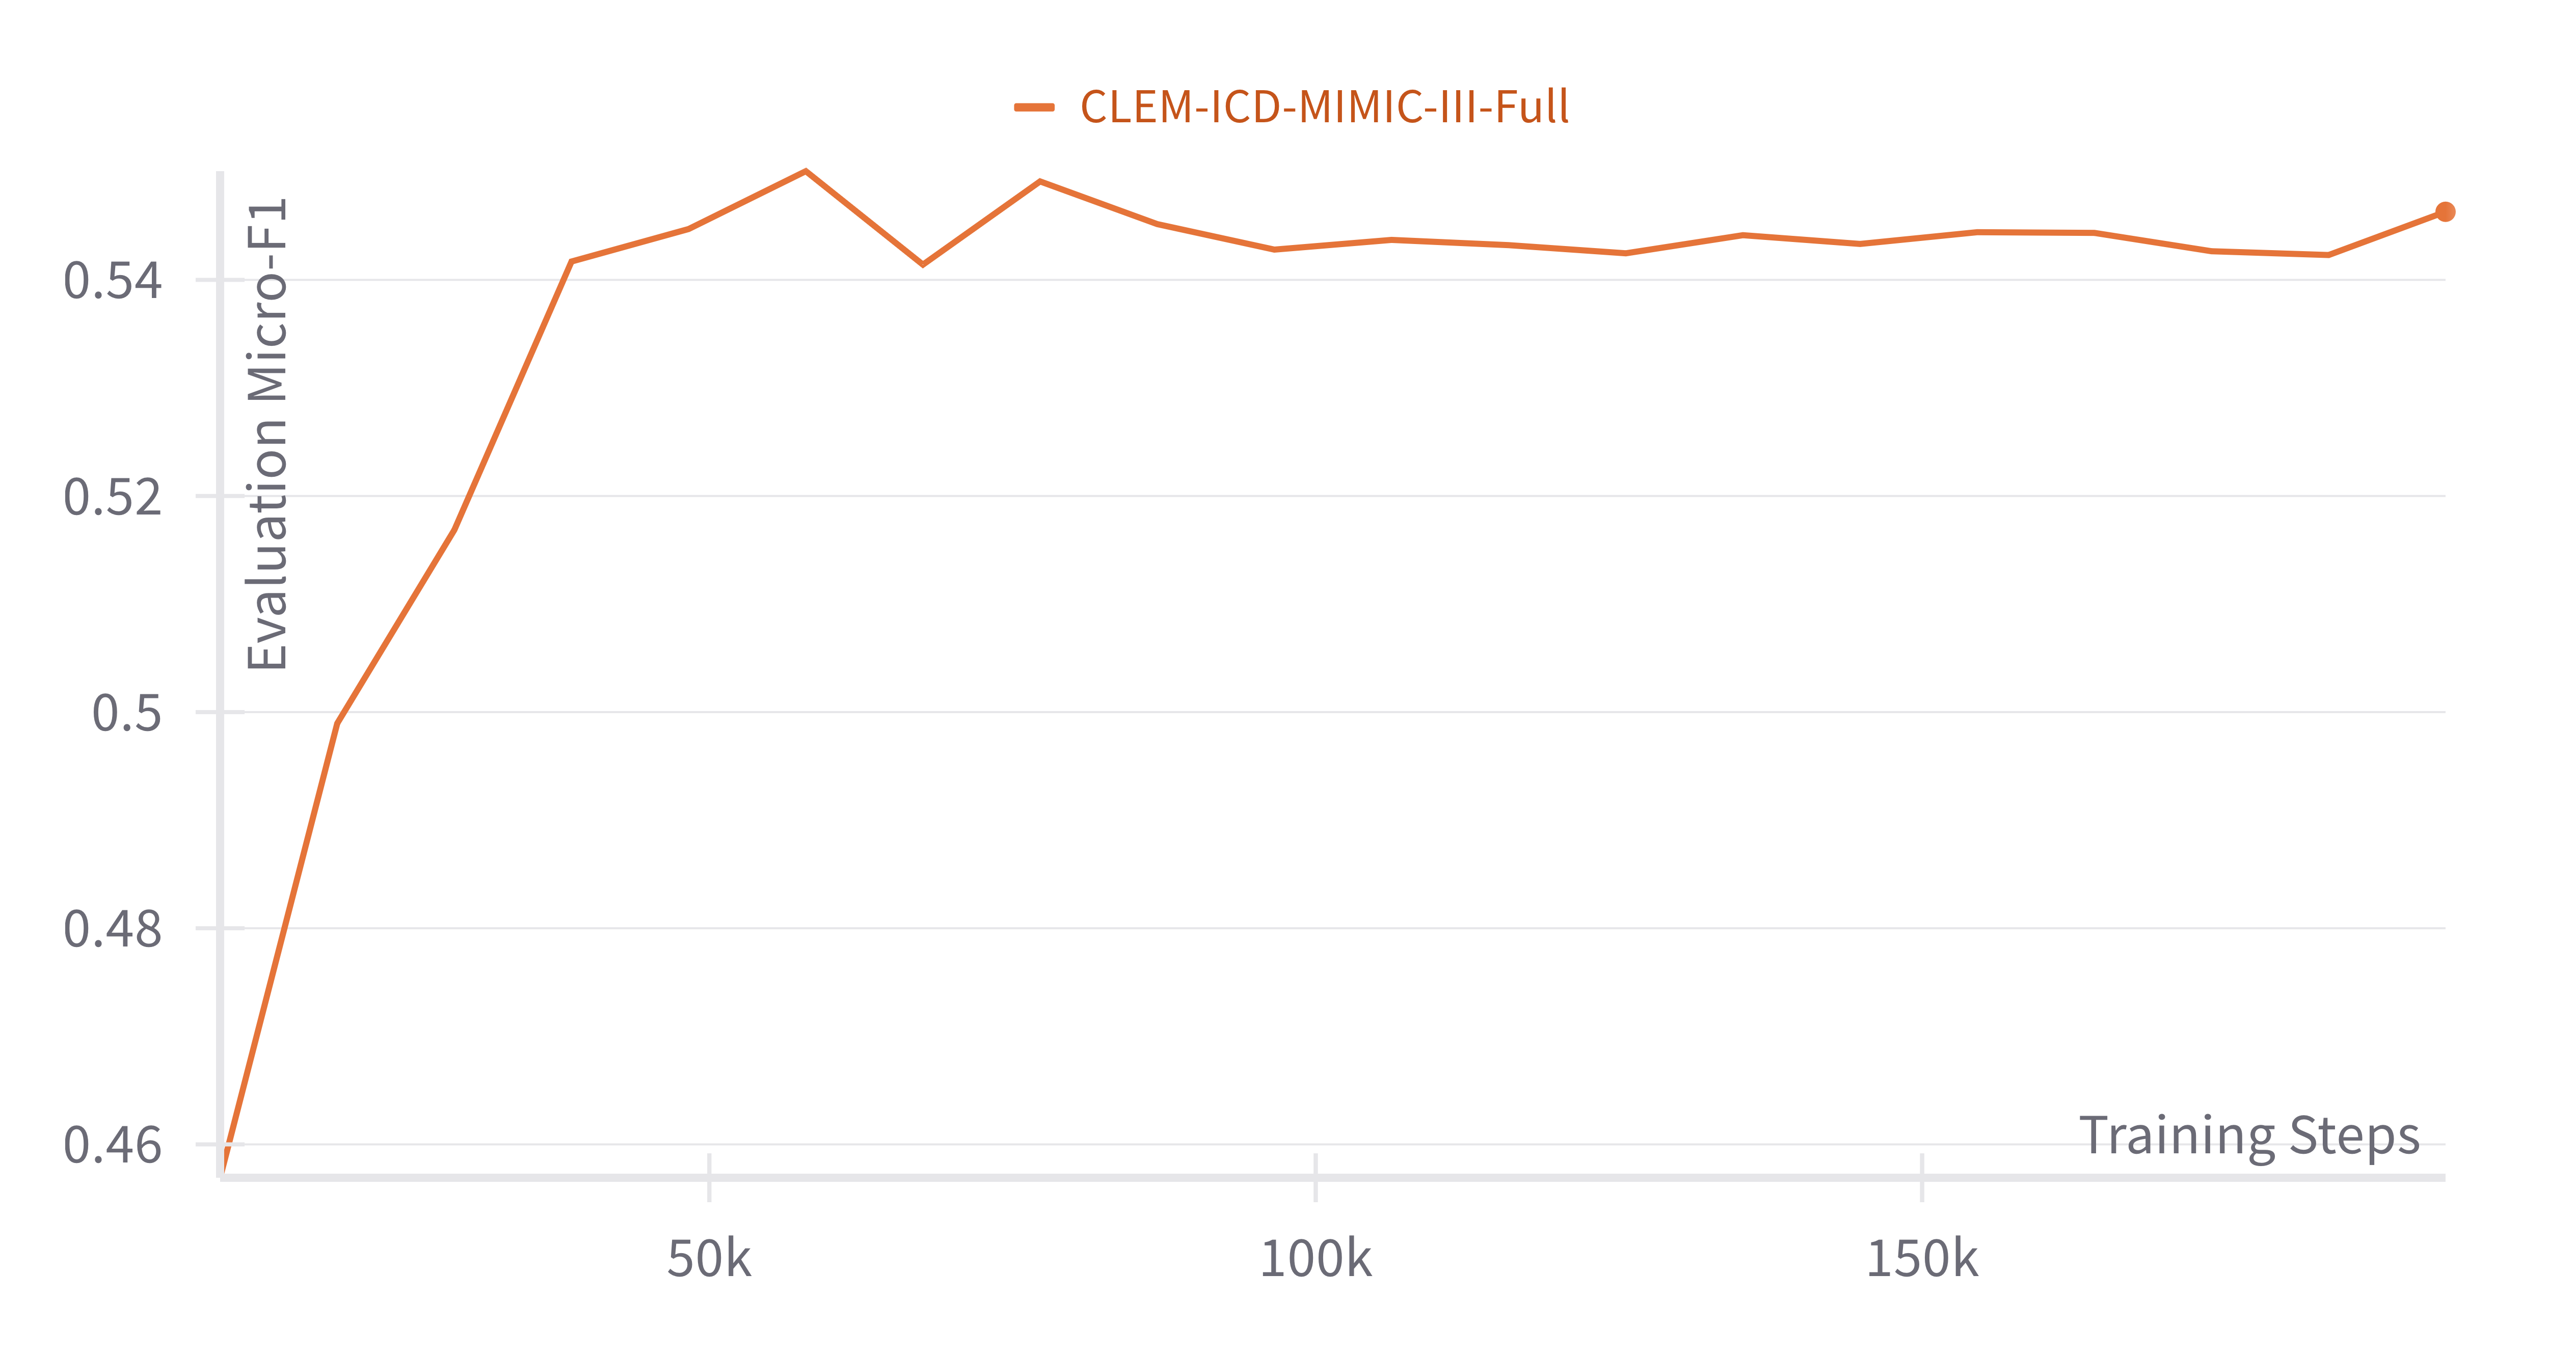
\includegraphics[keepaspectratio]{learning_curve_micro_f1_full.png}}

}

\subcaption{\label{fig-micro-f1-full}Evaluation Micro-F1 Score
(MIMIC-III Full)}

\end{minipage}%

\caption{\label{fig-learning-curves-full}Learning curves for CLEM-ICD
trained on the full MIMIC-III dataset (PLM-ICD splits) for 20 epochs.}

\end{figure}%

Observing the learning curves (Figure~\ref{fig-learning-curves-mdace}
and Figure~\ref{fig-learning-curves-full}), the model trained on the
full MIMIC-III dataset (Figure~\ref{fig-learning-curves-full}) appears
to plateau relatively early in training, particularly for Micro-F1,
while the model trained on the smaller MDACE split
(Figure~\ref{fig-learning-curves-mdace}) shows more continued
improvement later into the 10 epochs. Both runs exhibited signs of
overfitting, suggesting that future training could benefit from
implementing early stopping based on validation set performance.

\section{Discussion}\label{discussion}

\subsection{Architectural
Considerations}\label{architectural-considerations}

Our results underscore the advantage of leveraging transformer
architectures with natively long context windows for processing lengthy
clinical narratives in automated ICD coding. ModernBERT's 8192-token
capacity allows CLEM-ICD to process entire documents holistically,
potentially avoiding context fragmentation issues that can arise from
the segment pooling techniques employed by prior work like PLM-ICD
(Huang, Tsai, and Chen 2022) to handle shorter context limits. This
architectural choice significantly simplifies the implementation,
relying on standard Hugging Face library components
(\texttt{AutoModelForSequenceClassification}) rather than requiring
bespoke modules for segmentation or label-specific attention mechanisms,
which were critical for PLM-ICD's performance. While this standard
classification head might be considered less sophisticated than
specialized approaches for extreme multi-label classification (Chang et
al. 2019; Liu et al. 2024), the strong representational power of
ModernBERT combined with its ability to access the full document context
appears to compensate effectively for this task.

\subsection{Base Model Choice and
Efficiency}\label{base-model-choice-and-efficiency}

The selection of ModernBERT-base (Warner et al. 2024) as the foundation
model provides benefits beyond its extended context window.
Incorporating architectural optimizations adapted from recent
decoder-only models, ModernBERT-base (\textasciitilde138M parameters) is
designed for improved computational efficiency, demonstrating enhanced
inference speed compared to previous BERT-style encoders, particularly
for variable-length inputs and long sequences due to its alternating
attention mechanism (Warner et al. 2024). This increased efficiency
holds potential for deployment in settings with limited computational
resources or for enabling faster processing of large clinical datasets.
However, the base model utilized here underwent general-domain
pretraining (including text, code, and scientific literature) without
specific adaptation to clinical or biomedical language. Consequently,
further performance improvements might be realized through future
domain-specific adaptation, either via continued pretraining on clinical
corpora or fine-tuning biomedically-specialized ModernBERT variants.

\subsection{Performance Analysis and
Limitations}\label{performance-analysis-and-limitations}

The effectiveness of this approach is reflected in the competitive
results. CLEM-ICD achieves a superior Micro-F1 on the MDACE benchmark
compared to AttInGrad (Edin et al. 2024) and demonstrates a markedly
improved Macro-F1 score on the full MIMIC-III dataset compared to both
PLM-ICD (Huang, Tsai, and Chen 2022) and the more recent BL-5 model (Liu
et al. 2024). This strong Macro-F1 performance suggests that the model's
access to the full, unsegmented context and potentially the broader
knowledge within ModernBERT's pretraining data aids significantly in
classifying less frequent codes, a persistent challenge in this domain.
This capability is particularly relevant for developing coder assistance
tools, as human coders often need more support with rare codes than
common ones.

However, the lower Micro-F1 score on the full MIMIC-III dataset compared
to these benchmarks warrants consideration. This could be partly
attributed to factors like variance from a single training run or
differences in fine-tuning hyperparameters compared to the more
established benchmarks. The learning curves also indicated potential
overfitting (Figure~\ref{fig-learning-curves-mdace},
Figure~\ref{fig-learning-curves-full}), a known challenge when
fine-tuning large language models (Dodge et al. 2020), suggesting that
incorporating regularization techniques like early stopping is crucial.
Furthermore, this study deliberately focused on classification
performance. Consequently, it does not incorporate methods for enhancing
model interpretability, such as identifying supporting text spans (Cheng
et al. 2023) or visualizing attention patterns (Vaswani et al. 2017;
Edin et al. 2024), which remain important avenues for clinical NLP
research.

\section{Conclusion}\label{conclusion}

In this work, we presented CLEM-ICD, an automated ICD coding framework
leveraging the ModernBERT architecture. By utilizing ModernBERT's native
8192-token context window, CLEM-ICD processes lengthy clinical documents
effectively with a simplified architecture compared to previous methods
like PLM-ICD that required complex segmentation or attention mechanisms.
Our experiments demonstrate the potential of this approach, achieving
competitive performance on the MDACE benchmark and notably strong
Macro-F1 scores on the full MIMIC-III dataset, indicating improved
classification of less frequent codes. This work highlights the promise
of efficient, long-context encoder models for tackling the challenges of
automated medical coding. To support reproducibility and further
research, we release all code and model weights publicly.\footnote{Code
  and models available at
  \url{https://github.com/tylermarcuscross/explainable-medical-coding}}

\subsection{Future Work}\label{future-work}

Future research should focus on refining the fine-tuning process for
large-context models in this domain. Implementing robust early stopping
based on validation performance is a clear next step. Further
investigation into techniques specifically addressing the long-tail
distribution of ICD codes is warranted, including exploring specialized
loss functions or hierarchical classification strategies (Liu et al.
2024). Evaluating the efficacy of parameter-efficient fine-tuning (PEFT)
methods, such as LoRA (Hu et al. 2021), could also improve computational
feasibility and potentially mitigate overfitting. The public release of
our code and model weights aims to facilitate such investigations and
contribute to the broader goal of developing robust, efficient, and
potentially more interpretable automated medical coding systems.

\section*{References}\label{references}
\addcontentsline{toc}{section}{References}

\phantomsection\label{refs}
\begin{CSLReferences}{1}{0}
\bibitem[\citeproctext]{ref-chang2019taming}
Chang, Wei-Cheng, Hsiang-Fu Yu, Kai Zhong, Yiming Yang, and Inderjit S
Dhillon. 2019. {``Taming Pretrained Transformers for Extreme Multi-Label
Text Classification.''} In \emph{Proceedings of the 25th ACM SIGKDD
International Conference on Knowledge Discovery \& Data Mining},
318--28.

\bibitem[\citeproctext]{ref-cheng-etal-2023-mdace}
Cheng, Hua, Rana Jafari, April Russell, Russell Klopfer, Edmond Lu,
Benjamin Striner, and Matthew Gormley. 2023. {``MDACE: MIMIC Documents
Annotated with Code Evidence.''} In \emph{Proceedings of the 61st Annual
Meeting of the Association for Computational Linguistics}, 7534--50.
\url{https://doi.org/10.18653/v1/2023.acl-long.416}.

\bibitem[\citeproctext]{ref-dao2022flashattentionfastmemoryefficientexact}
Dao, Tri, Daniel Y. Fu, Stefano Ermon, Atri Rudra, and Christopher Ré.
2022. {``FlashAttention: Fast and Memory-Efficient Exact Attention with
IO-Awareness.''} \url{https://arxiv.org/abs/2205.14135}.

\bibitem[\citeproctext]{ref-dodge2020finetuning}
Dodge, Jesse, Gabriel Ilharco, Roy Schwartz, Ali Farhadi, Hannaneh
Hajishirzi, and Noah Smith. 2020. {``Fine-Tuning Pretrained Language
Models: Weight Initializations, Data Orders, and Early Stopping.''} In
\emph{arXiv Preprint arXiv:2002.06305}.

\bibitem[\citeproctext]{ref-edin2024explainable}
Edin, Joakim, Maria Maistro, Lars Maaløe, Lasse Borgholt, Jakob D.
Havtorn, and Tuukka Ruotsalo. 2024. {``An Unsupervised Approach to
Achieve Supervised-Level Explainability in Healthcare Records.''}
\emph{arXiv Preprint}. \url{https://arxiv.org/abs/2406.08958}.

\bibitem[\citeproctext]{ref-hu2021lora}
Hu, Edward J, Yelong Shen, Phillip Wallis, Zeyuan Allen-Zhu, Yuanzhi Li,
Shean Wang, Lu Wang, and Weizhu Chen. 2021. {``LoRA: Low-Rank Adaptation
of Large Language Models.''} In \emph{International Conference on
Learning Representations}.

\bibitem[\citeproctext]{ref-huang-etal-2022-plm}
Huang, Chao-Wei, Shang-Chi Tsai, and Yun-Nung Chen. 2022. {``PLM-ICD:
Automatic ICD Coding with Pretrained Language Models.''} In
\emph{Proceedings of the 4th Clinical Natural Language Processing
Workshop}, 10--20.
\url{https://doi.org/10.18653/v1/2022.clinicalnlp-1.2}.

\bibitem[\citeproctext]{ref-johnson2023mimic}
Johnson, Alistair E. W., Lucas Bulgarelli, Lu Shen, Alvin Gayles, Ayad
Shammout, Steven Horng, Tom J. Pollard, et al. 2023. {``MIMIC-IV, a
Freely Accessible Electronic Health Record Dataset.''} \emph{Scientific
Data} 10 (1): 1. \url{https://doi.org/10.1038/s41597-022-01899-x}.

\bibitem[\citeproctext]{ref-johnson2016mimic}
Johnson, Alistair EW, Tom J Pollard, Lu Shen, Li-Wei H Lehman, Mengling
Feng, Mohammad Ghassemi, Benjamin Moody, Peter Szolovits, Leo Anthony
Celi, and Roger G Mark. 2016. {``MIMIC-III, a Freely Accessible Critical
Care Database.''} \emph{Scientific Data} 3 (1): 1--9.

\bibitem[\citeproctext]{ref-kocher2011rethinking}
Kocher, Robert, and Nikhil R. Sahni. 2011. {``Rethinking Health Care
Labor.''} \emph{The New England Journal of Medicine} 365 (15): 1370--72.
\url{https://doi.org/10.1056/NEJMp1109649}.

\bibitem[\citeproctext]{ref-liu2023automated}
Liu, Leibo, Oscar Perez-Concha, Anthony Nguyen, Vicki Bennett, and
Louisa Jorm. 2024. {``Automated ICD Coding Using Extreme Multi-Label
Long Text Transformer-Based Models.''}

\bibitem[\citeproctext]{ref-tseng2018administrative}
Tseng, Phillip, Robert S. Kaplan, Barak D. Richman, Mahek A. Shah, and
Kevin A. Schulman. 2018. {``Administrative Costs Associated with
Physician Billing and Insurance-Related Activities at an Academic Health
Care System.''} \emph{JAMA} 319 (7): 691--97.
\url{https://doi.org/10.1001/jama.2017.19148}.

\bibitem[\citeproctext]{ref-vaswani2017attention}
Vaswani, Ashish, Noam Shazeer, Niki Parmar, Jakob Uszkoreit, Llion
Jones, Aidan N Gomez, Łukasz Kaiser, and Illia Polosukhin. 2017.
{``Attention Is All You Need.''} In \emph{Advances in Neural Information
Processing Systems}, 5998--6008.

\bibitem[\citeproctext]{ref-warner2024modernbert}
Warner, Benjamin, Antoine Chaffin, Benjamin Clavié, Orion Weller, Oskar
Hallström, Said Taghadouini, Alexis Gallagher, et al. 2024. {``Smarter,
Better, Faster, Longer: A Modern Bidirectional Encoder for Fast, Memory
Efficient, and Long Context Finetuning and Inference.''} \emph{arXiv
Preprint}. \url{https://arxiv.org/abs/2412.13663}.

\end{CSLReferences}




\end{document}
